% =====================================================================
% PRX Quantum submission: Regime-dependent quantum PINN benchmarking
% =====================================================================
% Compile: pdflatex main && bibtex main && pdflatex main && pdflatex main
% Or run: bash paper/build.sh
%
% Build status (P8 commit 1): SCAFFOLD ONLY. Title + abstract +
% section stubs. Numerical claims are added section-by-section in
% subsequent commits, with each cited number traced to a
% `results/` file via `scripts/verify_paper_integrity.py`.
% =====================================================================
\documentclass[%
  prx,
  twocolumn,
  amsmath,
  amssymb,
  aps,
  reprint,
  superscriptaddress,
  floatfix,
]{revtex4-2}

% Packages
\usepackage{graphicx}
\usepackage{booktabs}
\usepackage{hyperref}
\usepackage{xcolor}
\hypersetup{colorlinks=true,linkcolor=blue,citecolor=blue,urlcolor=blue}
\usepackage{siunitx}
\usepackage{microtype}

% Custom commands for our framework
\newcommand{\relltwo}{\mathrm{relL}^2}
\newcommand{\nsmooth}{n_{\mathrm{smooth}}}
\newcommand{\nbroad}{n_{\mathrm{broad}}}
\newcommand{\dsmooth}{\Delta_{\mathrm{smooth}}}
\newcommand{\dbroad}{\Delta_{\mathrm{broad}}}
\newcommand{\ddiff}{\Delta_{\mathrm{diff}}}
\newcommand{\qlnn}{QLNN}
\newcommand{\cpinn}{cPINN}

% Common abbreviations for system names
\newcommand{\fhn}{FitzHugh--Nagumo}
\newcommand{\lv}{Lotka--Volterra}
\newcommand{\vdp}{Van der Pol}
\newcommand{\ac}{Allen--Cahn}

\begin{document}

% Global glue-stretch budget. Two-column revtex with long ansatz
% names + nested math labels routinely produces 1-95pt overfull
% boxes that look fine in print but trigger noisy log warnings.
% Slightly looser inter-word stretch eliminates the cosmetic
% violations without affecting readability.
\sloppy
\emergencystretch=3em

% =====================================================================
% Title, authors, abstract
% =====================================================================
\title{%
  Regime-dependent advantage in quantum physics-informed neural
  networks: a pre-registered comparison on an ODE/PDE hardness
  ladder%
}

\author{Shawn Gibford}
\email{gibfords@gmail.com}
\affiliation{Independent}

\date{\today}

\begin{abstract}
We pre-register and execute a head-to-head benchmark of four quantum
physics-informed neural network (PINN) families against
capacity-matched classical PINN and Neural-ODE baselines, on a
hardness ladder of four ordinary and four partial differential
equations at three random seeds each. Following the methodology
proposed by Bowles, Ahmed, and Schuld for credible quantum
machine-learning benchmarks \textemdash{} matched training budgets,
paired-bootstrap confidence intervals, an underfit guard, and a
known-structure skyline \textemdash{} we test the pre-registered
hypothesis that quantum PINNs hold a regime-dependent advantage
favoring smooth/periodic over broadband/multiscale dynamics. The
hypothesis is FALSIFIED. Across both PRIMARY verdicts \textemdash{} the
full-ladder solver task at $n=24$ and the forecaster task at $n=9$
\textemdash{} the regime-dependent advantage is statistically
indistinguishable from zero, and the point estimate trends, if
anything, in the opposite (broadband-favoring) direction. One positive
sub-finding survives the falsification: the trainable-embedding quantum
PINN with a QNN encoder achieves markedly tighter seed-to-seed variance
and lower mean error than the matched classical PINN on stiff
fast--slow (\fhn{}) dynamics. We release the full open-source benchmark
framework, with every cited number mechanically verified against a
committed results file.
\end{abstract}

\maketitle

% =====================================================================
% Body sections — modular includes, one .tex per section
% =====================================================================
% Section: Introduction — P8 commit 2.
% Numerical claims verified against:
%   - results/p7_8_solver_h1_n24/h1_analysis_combined_n24.json
%   - results/p5_h1_verdict/h1_analysis.json
%   - results/p7_8_kdv_gate/gate_result.json
%   - ODE_PDE_PRE_REG.md (pre-registration)
%   - PRE_REG_AMENDMENT.md (A1--A11)
% All non-numerical claims are cited from refs in paper/references.bib.
% Methodology detail (BAS commitments, lineage, amendments, deferred
% Kuramoto/KdV extensions) lives in Methods (sec:methods); the intro
% states motivation, gap, what-we-did, the headline, and contributions.

\section{Introduction}
\label{sec:intro}

The question of whether variational quantum machine-learning (QML)
models offer a useful advantage over classical neural networks
remains contested~\cite{schuld2019quantum,havlicek2019supervised,
caro2022generalization}. Schuld and Killoran argue that the field
should pursue \emph{regime-dependent} advantages rather than blanket
quantum-supremacy claims~\cite{schuld2022right}: a quantum model is
``useful'' if it solves a specific class of problems better than the
best matched classical model at the same parameter budget.
Physics-informed neural networks (PINNs)~\cite{raissi2019physics,
karniadakis2021physics,lu2021deepxde} are a natural substrate for this
question, because the differential-equation residual loss is a single
scalar that depends on the model class through a clean
derivative-of-parameterized-function interface and admits
capacity-matched classical baselines. The emerging family of
\emph{quantum PINNs}~\cite{perezsalinas2020dataru,kyriienko2021solving,
markidis2022physics,berger2025teqpinn,sedykh2024quantum,
farea2025qcpinn,ahmed2024rfqrc} carries a theoretically motivated
regime-dependence claim: the data-reuploading Fourier series accessible
to a quantum circuit~\cite{schuld2021effect} should grant an inductive
bias for smooth, periodic dynamics. Yet the empirical picture is
fragmentary --- most quantum-PINN papers report a single task, often
without matched classical baselines or pre-registered acceptance
criteria --- leaving the central question \emph{when, and on what kinds
of problems, does a quantum PINN outperform a capacity-matched
classical PINN?} unanswered at any rigorous level.

Bowles, Ahmed, and Schuld recently catalogued the methodological gaps
that make QML benchmarks unreliable~\cite{bowles2024better,
huang2021power} --- undertuned classical baselines, mismatched
parameter counts, best-of-many-seeds reporting, and isolated wins in
place of statistically defensible contrasts --- and propose a set of
commitments (pre-registration, matched budgets, paired-bootstrap
inference, an underfit guard, and a known-structure skyline) that any
advantage claim should satisfy. To our knowledge, no published
quantum-PINN benchmark has implemented this framework on a hardness
ladder spanning both ordinary and partial differential equations. This
paper does so.

Following a pre-registration committed before any results were
generated (Methods~\ref{sec:methods}; Appendix~A), we test the
hypothesis that quantum PINNs achieve a regime-dependent advantage on
smooth/periodic versus broadband/multiscale dynamical systems. Four
quantum-PINN families --- data-reuploading~\cite{perezsalinas2020dataru},
the trainable-embedding QPINN with classical-FNN and with QNN
encoders~\cite{berger2025teqpinn}, and the hybrid
QCPINN~\cite{farea2025qcpinn} --- are run against capacity-matched
classical PINN and non-liquid Neural-ODE baselines on four ODEs
(\lv{}, \vdp{}, Lorenz, \fhn{}) and four PDEs (heat, smooth Burgers,
\ac{}, shock Burgers) at three seeds each (24 cells total), with every
system pre-registered as smooth/periodic or broadband/multiscale.

\textbf{The pre-registered hypothesis is FALSIFIED.} The solver-task
PRIMARY verdict at $n=24$ is $\ddiff = \dsmooth - \dbroad = -0.084$
(paired-bootstrap 95\% CI $[-0.278, +0.061]$, including zero), and the
forecaster-task PRIMARY verdict at $n=9$ is $\ddiff = -0.501$ (CI
$[-0.804, -0.244]$, excluding zero in the \emph{broadband-favoring}
direction). Three additional sensitivity points --- a default-Adam
combined verdict, a both-sides hyperparameter-optimized verdict, and
the original-pre-registration forecaster verdict
(Section~\ref{sec:verdict}) --- return the same qualitative result. The
point estimate even flips sign as the broadband bin is expanded from
six to twelve cells, hinting (without statistical significance) at the
\emph{inverse} of the original hypothesis. The robust conclusion is the
absence of a statistically distinguishable regime-dependent
quantum-PINN advantage at this matched-capacity, matched-budget scale.

Within the falsification, the expanded ladder surfaces one positive
sub-finding worth reporting on its own terms. On \fhn{}, the
trainable-embedding quantum PINN with QNN encoder
(\texttt{te\_qpinn\_qnn})~\cite{berger2025teqpinn} attains a
seed-to-seed standard deviation roughly twenty-four times tighter and a
seed-mean error roughly two-and-a-half times lower than the matched
classical PINN (Section~\ref{sec:solver}) --- a regime-specific
structural edge on stiff fast--slow dynamics, achieved with zero
classical parameters in the ansatz and at the same training budget as
every other cell.

The paper's contributions are fourfold. \emph{Methodologically}, it
delivers an open-source quantum-PINN benchmarking framework that
implements the full Bowles--Ahmed--Schuld
protocol~\cite{bowles2024better} --- pre-registration with falsifiable
acceptance rules, matched parameter budgets, paired-bootstrap
inference, underfit and skyline guards, and symmetric hyperparameter
sensitivity --- backed by a script that mechanically gates every cited
number against a committed JSON file, with twenty-two pre-registration
amendments documented openly (Appendix~A). \emph{Empirically}, it
falsifies the regime-dependent advantage hypothesis across two PRIMARY
verdicts and three layered sensitivity points, covering all eight
hardness-ladder systems and both pre-registered tasks, while
identifying the \texttt{te\_qpinn\_qnn} structural sub-finding at
matched compute. \emph{Mechanistically}, it cross-tabulates the
per-cell advantage gap against trainability and expressivity scalars
(Kullback--Leibler divergence to a Haar-random ensemble, accessible
Fourier $K_{\max}$~\cite{schuld2021effect}, and gradient variance),
finding a leave-one-out-robust but underpowered trend consistent with
the inverted pattern (Section~\ref{sec:mechanism}). Finally, the full
code, data, and reproduction pipeline are released at
\url{https://github.com/shawngibford/qlnn}, with the reproducibility
commitments following NeurIPS program guidance~\cite{pineau2021improving}.

\subsection*{What this paper does \emph{not} claim}

To be precise about scope: this paper does not claim a quantum
advantage; it claims its \emph{absence} at this matched-capacity,
matched-budget scale. It does not claim that the H1 hypothesis is false
in general --- only that the pre-registered acceptance threshold is not
crossed on this hardness ladder. It does not claim that the
broadband-leaning point estimate sign is reliable; the confidence
interval crosses zero on every solver-side sensitivity point. And it
does not assert generalization from $n=24$ cells to the full QML/PDE
landscape; the follow-up experiments named in
Section~\ref{sec:discussion} are precisely what that would require.

The rest of the paper proceeds as follows: Methods
(Section~\ref{sec:methods}), solver- and forecaster-task results
(Sections~\ref{sec:solver}--\ref{sec:forecaster}), the aggregated H1
verdict and sensitivity analysis (Section~\ref{sec:verdict}), the
mechanism cross-tabulation (Section~\ref{sec:mechanism}), and
discussion and conclusions
(Sections~\ref{sec:discussion}--\ref{sec:conclusions}).

% Section: Methods — P8 commit 3.
% Numerical claims verified against:
%   - ODE_PDE_PRE_REG.md §§ 1-7
%   - PRE_REG_AMENDMENT.md A1--A11
%   - src/quantum_liquid_neuralode/evaluation/h1_verdict.py
%   - src/qlnn_/training/{pde_residual_loss, multi_state_solver,
%       classical_pinn_solver, p3_8_review_demo, p3_9_pde_matrix}.py
%   - Per-cell metrics.json (param counts)

\section{Methods}
\label{sec:methods}

\subsection{Pre-registration and the falsifiable hypothesis}
\label{sec:methods-prereg}

The complete pre-registration document (\texttt{ODE\_PDE\_PRE\_REG.md},
committed 2026-05-19 before any benchmark results were generated)
states the central hypothesis:

\begin{quote}
\textbf{H1.} Quantum PINNs achieve a regime-dependent advantage over
matched classical baselines: $\dsmooth - \dbroad > 0$ with
paired-bootstrap 95\% confidence interval excluding zero, where
$\Delta_\text{cell} \equiv \relltwo_\text{classical} -
\relltwo_\text{QLNN}$ and the mean is taken per regime.
\end{quote}

The theoretical motivation is the Schuld--Sweke--Meyer
result~\cite{schuld2021effect} that a data-reuploading parameterized
quantum circuit realizes a truncated Fourier series in the encoded
variable, with accessible $K_\text{max}$ proportional to reuploading
depth. A model whose hypothesis class is a low-order Fourier series
should exhibit an inductive bias toward smooth periodic dynamics and
a corresponding difficulty representing broadband or multiscale
structure. H1 operationalizes this prediction as a comparison
between two pre-registered regime bins.

The pre-registration locks three additional commitments before
any result is generated: (i)~mandatory classical baselines
(capacity-matched cPINN, non-liquid Neural-ODE, plain MLP
forecaster, and a known-structure skyline); (ii)~banned headline
metrics that admit persistence-trivial wins (notably one-step MAE
on autoregressive rollout); (iii)~explicit decision rules under
which H1 is declared CONFIRMED, FALSIFIED, or INCONCLUSIVE.

Nineteen amendments to the pre-registration are documented openly
in \texttt{PRE\_REG\_AMENDMENT.md} (A1--A19). They were necessary
because the original pre-registration left some parameter choices
implicit; each amendment locks a single decision and reports
whether the outcome was stable under the alternative choice. The
key amendments from the original analysis pass are: A1 (skyline
threshold = 0.5; sensitivity at 0.75 reported); A4 (MLP capacity
3.3$\times$ Neural-ODE, violating the original ``within factor of
2'' rule, disclosed and shown not to affect the verdict sign); A7
(strict-versus-raw underfit-guard reporting); A9 (symmetric
quantum HPO sensitivity); A10 (combined ODE+PDE verdict at
$n=18$); A11 (full-ladder expansion to $n=24$ + KdV/Kuramoto
deferral rationale). Amendments A15--A19 were filed 2026-05-28
during an internal audit that surfaced (a) cross-side
training-budget parity across all solver models, (b) a PennyLane
\texttt{StronglyEntanglingLayers} fallback that silently aliased
\texttt{data\_reuploading} at the project's qubit count, (c) a
\texttt{qcpinn} quantum-attribution sub-experiment with three
step-wise variants, (d) \texttt{brickwall}'s structural
connectivity deficit at small qubit count (removed from the
empirical sweep; T3 mechanism scalars retained as
untrained-circuit diagnostic data), and (e) cross-task
forecaster/solver training-step budget parity. The verdict
refresh under the A15--A19 configuration is deferred to a
supplementary compute campaign; the verdicts reported in this
manuscript reflect the configuration locked at the time of
analysis.

\subsection{Hardness ladder}
\label{sec:methods-ladder}

We test H1 on eight pre-registered dynamical systems organized
into a regime-tagged hardness ladder.

\textbf{Smooth/periodic bin} (six pre-reg cells, four taxa, two
mathematical structures):
\begin{itemize}
  \item \lv{} ($\alpha = 1.1, \beta = 0.4, \delta = 0.1,
        \gamma = 0.4$, $T = 5$) -- 2D predator--prey limit cycle.
  \item \vdp{} ($\mu = 5$, $T = 10$) -- 2D stiff but periodic
        relaxation oscillator; pre-registered as borderline
        smooth.
  \item Heat equation ($\nu = 0.1$, $T = 1$, periodic
        on $[0, 2\pi)$) -- analytic reference
        $u(t,x) = e^{-\nu t}\sin x$.
  \item Burgers smooth ($\nu = 0.12$, $T = 2$, periodic on
        $[0, 2\pi)$, IC $\sin x$) -- npz-reference field.
\end{itemize}

\textbf{Broadband/multiscale bin} (six pre-reg cells, four taxa,
two mathematical structures):
\begin{itemize}
  \item Lorenz ($\sigma = 10, \rho = 28, \beta = 8/3$, $T = 2$)
        -- 3D chaotic flow.
  \item \fhn{} ($I = 0.5, \varepsilon = 0.08, a = 0.7, b = 0.8$,
        $T = 20$) -- 2D fast--slow stiff relaxation.
  \item \ac{} ($\varepsilon = 0.06$, $T = 8$, periodic on
        $[0, 2\pi)$) -- sharp two-front equilibrium.
  \item Burgers shock ($\nu = 0.004$, $T = 2$, periodic on
        $[0, 2\pi)$, IC $\sin x$) -- near-shock at $t^* \approx 1$.
\end{itemize}

Two pre-registered systems are mechanism-proven-but-compute-deferred
(amendment A11): the 12-dimensional Kuramoto coupled-oscillator
system (per-component scalar circuits scale linearly in state
dimension, projecting $\approx 7$~hr per cell) and KdV
($u_t + 6 u u_x + u_{xxx} = 0$). The triple-nested reverse-mode
autodiff required for the KdV solver was gate-tested
(\texttt{scripts/run\_p7\_8\_kdv\_gate.py}, result:
PASS, $u_{xxx}$ values finite and nontrivial, JIT compile
4.55~s, per-point cost ratio 0.431$\times$ the second-order
baseline thanks to XLA fusion); the integrated training cost at
$32 \times 32$ collocation and 2400 steps remains prohibitive
($\approx 12$~s per gradient step, projecting $\approx 8$~hr
per seed across all four quantum families plus the classical
baseline). Both deferrals are queued for the follow-up paper.

\subsection{Quantum-PINN family roster}
\label{sec:methods-roster}

Four quantum-PINN ansatz families are exercised at all 24 cells.
Each family is implemented faithfully against its published
specification; the binding manifest is
\texttt{refs/CIRCUIT\_SPECS.md}. For solver-task ODEs, each $d$-component
state is fitted via $d$ independent scalar circuits with $d$
separate weight pytrees (no entanglement across components); for
PDEs, each family has a 2D port that encodes $(t, x)$ on split
qubit registers.

\begin{itemize}
  \item \textbf{Data-reuploading} (Pérez-Salinas et
        al.~\cite{perezsalinas2020dataru}): the universal
        classifier ansatz with interleaved angle-encoding and
        parameterized $R(\theta)$ blocks plus ring CNOT
        entanglers. 4 qubits, 5 layers, 60 PQC parameters per
        scalar circuit.
  \item \textbf{TE-QPINN/FNN} (Berger et
        al.~\cite{berger2025teqpinn}): trainable-embedding QPINN
        with classical FNN encoder feeding angle-encoded rotations.
        60 PQC parameters and 100 classical FNN parameters per
        scalar circuit.
  \item \textbf{TE-QPINN/QNN} (Berger et
        al.~\cite{berger2025teqpinn}): trainable-embedding QPINN
        with QNN encoder (zero classical parameters by
        construction). 84 PQC parameters per scalar circuit.
  \item \textbf{QCPINN} (Farea et
        al.~\cite{farea2025qcpinn}): hybrid quantum--classical
        PINN with classical pre- and post-net. 15 PQC parameters
        and 706 classical parameters per scalar circuit (the
        classical-parameter overhead is disclosed openly and
        flagged at every cell in the per-cell tables in
        Section~\ref{sec:solver}).
\end{itemize}

For all four families the 2D PDE port uses split qubit registers:
$n_t = n_x = 4$ qubits per coordinate axis, 5 hardware-efficient
layers, ring entanglement. The Chebyshev coordinate feature map
realizes a tower of Chebyshev polynomials in each axis variable;
the convention is \texttt{src/qlnn\_/training/pde\_residual\_loss.py}
\texttt{ChebyshevDQC2DConfig}.

\subsection{Matched classical baselines}
\label{sec:methods-baselines}

Per pre-registration §6 (mandatory), four classical baselines are
trained at every applicable cell at matched parameter count
within a factor of two (except A4-disclosed MLP):

\begin{itemize}
  \item \textbf{Classical PINN} (cPINN): a small MLP trained with
        the same Lagaris hard-IC trial solution
        $u(t, x) = u_0(x) + (t - t_0) \cdot \text{MLP}_\theta(t, x)$
        and the same physics residual as each quantum-PINN cell.
        For vector ODE: $u(t) = u_0 + (t - t_0) \cdot \text{MLP}(t)$
        with output dimension $d$. The classical solver-task control.
  \item \textbf{Plain non-liquid Neural-ODE}: an MLP cell
        $h' = W_{\text{out}}\tanh(W_h [h, x, t])$ with no learnable
        time constants, Diffrax integration, the same residual head
        as the quantum forecaster. The forecaster-task control.
  \item \textbf{Plain MLP forecaster}: $y = \text{MLP}(\text{history}, x)$
        as a capacity-matched non-recurrent forecaster control.
  \item \textbf{Known-structure skyline}: per pre-reg §6, fits only
        free coefficients (e.g.~$\nu$, $\rho$) of the ground-truth
        equation by least squares against the reference trajectory.
        Used as the underfit/out-of-reach gate.
\end{itemize}

\subsection{Training protocol}
\label{sec:methods-train}

All solver-task cells use the Lagaris hard-IC trial solution. The
ODE form is $u(t) = u_0 + (t - t_0) \cdot (s \cdot
\text{circuit}(t) + b)$ with $\{s, b\}$ scalar training parameters
per component; the PDE form is
$u(t, x) = u_0(x) + (t - t_0) \cdot
(s \cdot \text{circuit}(t, x) + b)$. The physics-residual loss is
the mean squared residual over interior collocation points;
all four quantum-PINN families and the classical PINN share the
same loss closure, so the comparison differs only in the function
class of the trial solution.

Per-axis collocation grids: 60 interior points for ODE solvers, and
either $24{\times}24$, $28{\times}28$, or $32{\times}32{-}64$
for PDE solvers (the AC and burgers\_shock grids are intentionally
finer to capture the sharper structures, per A11). Training step
budgets per system are documented in
\texttt{CORRECTED\_PDE\_CONFIGS}: 1200 for heat, 1500 for
burgers\_smooth, 1800 for AC, 2400 for burgers\_shock. ODE step
budgets follow \texttt{multi\_state\_solver.\_SCALAR\_FAMILIES}:
1200 (chebyshev\_dqc), 1500 (te\_qpinn\_fnn, qcpinn), 2000
(te\_qpinn\_qnn).

\subsection{Verdict machinery}
\label{sec:methods-verdict}

Per cell the trained model is evaluated on an interior 50$\times$50
grid (PDE) or a 1024-point time grid (ODE), and we record
relative-$L^2$ error against the reference field. We construct one
\texttt{CellRecord} per (system, seed) with the best quantum-PINN
relative-$L^2$ across the four families on the quantum side and
the matched classical-PINN result on the classical side. The H1
verdict module (\texttt{h1\_verdict.py} in the
\texttt{quantum\_liquid\_neuralode.evaluation} package) performs
the following:

\begin{enumerate}
  \item \emph{Underfit guard}: drops cells where the classical
        baseline fails to reach an adequacy threshold (its train-side
        $\relltwo > 0.5$ under A7's strict reading).
  \item \emph{Skyline guard}: drops cells where the known-structure
        skyline cannot itself reach the adequacy threshold.
        At threshold 0.5 (A1), all skyline cells pass.
  \item \emph{Paired-bootstrap}: resamples the kept cells with
        replacement, computing per-resample $\dsmooth$ and
        $\dbroad$, and reports the percentile 95\% CI of
        $\ddiff = \dsmooth - \dbroad$. Default $n_{\text{iter}} =
        10{,}000$, $\alpha = 0.05$.
  \item \emph{Decision rule}: CONFIRMED if the CI excludes zero
        positively; FALSIFIED if it includes zero or excludes
        zero negatively; INCONCLUSIVE if the guards drop too
        many cells to render the bootstrap underpowered.
\end{enumerate}

The pre-registration commits the framework to mechanical
application of these rules; no analyst chooses the verdict
post-hoc.

\subsection{Symmetric HPO sensitivity}
\label{sec:methods-hpo}

Amendment A9 adds a symmetric quantum-side hyperparameter sweep
that mirrors the classical-side sweep already in
\texttt{run\_p7\_5\_hpo\_sensitivity.py}. At three anchor cells
(\lv{} seed~2, \vdp{} seed~1, Lorenz seed~2), each
of the four quantum families is retrained at three learning
rates $\{10^{-3}, 5 \cdot 10^{-3}, 10^{-2}\}$ and two training
budgets $\{1500, 3000\}$ steps -- 72 retrains in total. The
``full HPO-best'' verdict reported in Section~\ref{sec:verdict}
takes the per-cell minimum-$\relltwo$ HPO point on both sides.
This is the Bowles--Schuld~\cite{bowles2024better} ``tune both
sides'' sensitivity test.

\subsection{Open-source reproducibility}
\label{sec:methods-repro}

The repository at
\url{https://github.com/shawngibford/qlnn} contains the complete
code, pre-registration, and committed result JSONs.
\texttt{scripts/reproduce\_paper.sh} regenerates every committed
result from scratch (estimated wall-clock $\approx$~8~hr on a
single MacBook Pro M1, parallelizable);
\texttt{scripts/verify\_paper\_integrity.py} mechanically checks
every cited number in this paper against its committed JSON file
and returns non-zero if any number drifts. Tagged GitHub releases
mark the post-rigor (\texttt{v0.1-prepaper-rigor}) and
post-airtight-matrix (\texttt{v0.2-airtight-matrix}) checkpoints.

% Section: Solver-task results — filled in P8 commit 4.
\section{Solver-task results}
\label{sec:solver}
\noindent\emph{[Section stub. Drafted in P8 commit 4.]}

% Section: Forecaster-task results — P8 commit 5.
% All numerical claims verified against:
%   - results/p4_forecaster_rollout/{system}_{family}/seed_N/metrics.json
%   - results/p5_matched_baselines/{system}_{baseline}/seed_N/metrics.json
%   - results/p7_10_forecaster_decomposition/per_cell_records.json
%   - results/p7_10_forecaster_decomposition/h1_*.json
%   - results/p5_h1_verdict/h1_analysis.json
% Decomposition rationale: PRE_REG_AMENDMENT A12.

\section{Forecaster-task results}
\label{sec:forecaster}

The forecaster task is the corroborating verdict per pre-reg \S7:
each model learns an autoregressive one-step predictor from a
training trajectory and is evaluated on its multi-step rollout
against a held-out test trajectory. The pre-registered $H_1$
contrast pits the QLNN forecaster against the non-liquid
Neural-ODE baseline, but the QLNN forecaster has learnable
per-qubit time constants $\tau$ (the
\texttt{LiquidQuantumCell}) that the baseline lacks. Per amendment
A12 (P7.10), we add the missing fourth-quadrant baseline -- a
classical liquid-time-constant forecaster
(\texttt{ClassicalLTCForecaster},
Hasani-form~\cite{hasani2021liquid} with no quantum circuit) -- so
the verdict decomposes cleanly into the quantum and liquid-$\tau$
contributions that the original contrast confounds.

\subsection{All-to-all per-cell error matrix}
\label{sec:forecaster-cells}

Table~\ref{tab:forecaster-matrix} reports the per-cell relative-$L^2$
rollout error for the full all-to-all contrast: five quantum
forecaster families (the four registry ansätze plus the SOTA
recurrence-free quantum reservoir
\texttt{rf\_qrc}~\cite{ahmed2024rfqrc}) against four classical
baselines (\texttt{plain\_neuralode}, \texttt{plain\_mlp}, the
\texttt{skyline} fitting the known structural RHS by least
squares, and the P7.10 \texttt{classical\_ltc}), across all nine
ODE cells (3 systems $\times$ 3 seeds).

\begin{table*}[t]
\centering
\caption{All-to-all per-cell relative-$L^2$ rollout error on the
$n=9$ forecaster matrix. Five quantum forecaster families
$\times$ four classical baselines. The architectural family names
abbreviate to: ``dataru'' for \texttt{data\_reuploading},
``hweff'' for \texttt{hardware\_efficient}, ``stngent'' for
\texttt{strongly\_entangling} (which aliases to the
\texttt{data\_reuploading} circuit in our registry; the column is
kept for all-to-all transparency), ``brick'' for \texttt{brickwall},
``rfqrc'' for \texttt{rf\_qrc}. Classical baselines:
``ne'' for \texttt{plain\_neuralode} (the pre-reg-mandated H1
contrast), ``mlp'' for \texttt{plain\_mlp}, ``sky'' for
\texttt{skyline}, ``ltc'' for the P7.10
\texttt{classical\_ltc}. Bold marks the best quantum and best
classical model on that row.}
\label{tab:forecaster-matrix}
\scriptsize
\setlength{\tabcolsep}{3pt}
\begin{tabular}{lc|ccccc|cccc}
\toprule
System & Seed & dataru & hweff & stngent & brick & rfqrc &
ne & mlp & sky & ltc \\
\midrule
\multicolumn{11}{l}{\emph{Smooth/periodic:}} \\
\lv{}     & 0 & 0.577 & 0.680 & 0.577 & 0.863 & 1.046 &
                \textbf{0.288} & 0.754 & \textbf{0.020} & 0.230 \\
\lv{}     & 1 & 0.761 & \textbf{0.537} & 0.761 & 0.751 & 0.893 &
                \textbf{0.299} & 0.561 & 0.020 & 0.209 \\
\lv{}     & 2 & 0.813 & 0.696 & 0.813 & \textbf{0.327} & 1.079 &
                \textbf{0.471} & 0.694 & 0.020 & 0.659 \\
\vdp{}    & 0 & 1.330 & \textbf{1.274} & 1.330 & 9.607 & 1.410 &
                \textbf{1.389} & 13.729 & 0.962 & 1.363 \\
\vdp{}    & 1 & 8.352 & \textbf{1.201} & 8.352 & 11.107 & 1.626 &
                \textbf{1.236} & 2.741 & 0.962 & 1.216 \\
\vdp{}    & 2 & \textbf{1.192} & 1.221 & 1.192 & 4.091 & 4.246 &
                \textbf{1.217} & 2.577 & 0.962 & 1.216 \\
\midrule
\multicolumn{11}{l}{\emph{Broadband/multiscale:}} \\
Lorenz    & 0 & 1.027 & 0.986 & 1.027 & 1.343 & \textbf{0.607} &
                \textbf{0.943} & 1.919 & 0.708 & 0.855 \\
Lorenz    & 1 & 0.519 & \textbf{0.485} & 0.519 & 0.494 & 0.841 &
                \textbf{0.758} & 1.872 & 0.708 & 0.788 \\
Lorenz    & 2 & 1.185 & 0.612 & 1.185 & 1.614 & \textbf{0.460} &
                \textbf{1.248} & 0.805 & 0.708 & 1.650 \\
\bottomrule
\end{tabular}
\end{table*}

Three patterns stand out in the all-to-all matrix.

\textbf{(1) The skyline is structurally exceptional on \lv{}.}
The known-RHS least-squares skyline attains $\relltwo = 0.020$
across all three \lv{} seeds -- two orders of magnitude better
than any learned model. This is the structural cap the skyline
guard (Section~\ref{sec:methods-verdict}) exists to surface:
\lv{} is at-reach, and any learned model that loses to the skyline
by an order of magnitude has a real gap to close. The pattern
holds on Lorenz ($\relltwo \approx 0.71$) but weakens on \vdp{}
($\relltwo \approx 0.96$, near the predict-zero floor).

\textbf{(2) Classical baselines mostly beat the
quantum families on smooth ODEs.}
On \lv{}, the strongest learned model is consistently
\texttt{plain\_neuralode} or \texttt{classical\_ltc}, beating the
best quantum family by a clear margin on two of three seeds. On
\vdp{}, all models sit far above the predict-zero floor
($\relltwo > 1$), several quantum cells blowing up catastrophically
(\texttt{data\_reuploading} s1: $8.35$; \texttt{brickwall} s0:
$9.61$; \texttt{plain\_mlp} s0: $13.73$). \vdp{} at $\mu=5$
is near the learnability boundary for matched-capacity models on
the pre-registered rollout horizon.

\textbf{(3) The quantum families show their advantage on Lorenz.}
\texttt{rf\_qrc} attains the best Lorenz s0 ($0.607$) and s2
($0.460$) cells, outperforming both the matched classical
baselines and the other quantum families;
\texttt{hardware\_efficient} wins Lorenz s1 ($0.485$). This is the
broadband-chaotic regime where the solver-task expansion (\fhn{},
\ac{}) also surfaced regime-specific quantum advantages --
consistent across both tasks, even though the global $H_1$ verdict
here is FALSIFIED.

\subsection{Combined verdict and LTC decomposition}
\label{sec:forecaster-decomp}

The pre-reg-mandated combined verdict selects the best quantum
family per cell as the QLNN representative and runs the
paired-bootstrap $H_1$ verdict against \texttt{plain\_neuralode}
(Section~\ref{sec:methods-verdict}). Per amendment A12, we add two
decomposition verdicts that share the cell records but swap which
baseline sits in the contrast slot:

\begin{align*}
\Delta_\mathrm{cmb} &= \mathrm{QLNN} - \text{Neural-ODE} \\
\Delta_q  &= \mathrm{QLNN} - \text{cLTC} \\
\Delta_\tau   &= \text{cLTC} - \text{Neural-ODE}
\end{align*}

The per-cell algebraic identity $\Delta_\mathrm{cmb} =
\Delta_q + \Delta_\tau$ holds exactly
(verified mechanically in
\texttt{verify\_paper\_integrity.py}; tolerance $10^{-3}$).

\begin{table}[h]
\centering
\caption{Forecaster-task $H_1$ decomposition at $n=9$ cells. All
three verdicts are FALSIFIED. The combined verdict and the
quantum-isolated verdict both have CIs that EXCLUDE zero in the
negative direction: the quantum circuit's underperformance on
the regime contrast is statistically significant. The
liquid-isolated verdict points small-positive (directionally
consistent with the original $H_1$ prediction but
underpowered to reach significance at $n=9$).}
\label{tab:forecaster-decomp}
\small
\begin{tabular}{lrll}
\toprule
Verdict & $\ddiff$ & 95\% CI & Outcome \\
\midrule
Combined         & $-0.501$ & $[-0.804, -0.244]$ & FALSIFIED \\
\textbf{Quantum-isolated} & $\mathbf{-0.616}$ & $\mathbf{[-1.167, -0.178]}$ &
  FALSIFIED \\
Liquid-isolated  & $+0.115$ & $[-0.097, +0.377]$ & FALSIFIED \\
\bottomrule
\end{tabular}
\end{table}

The decomposition tells a clear mechanism story.

\textbf{The quantum circuit is the source of the regime-contrast
underperformance, at high statistical confidence.} The
quantum-isolated CI $[-1.167, -0.178]$ EXCLUDES zero negatively:
the quantum circuit's contribution to $\ddiff$ is significantly
negative. Under matched-capacity training, quantum forecasters
underperform classical-LTC more on smooth ODEs than on broadband.
The combined point estimate ($-0.501$) is less negative than the
quantum-isolated estimate ($-0.616$) because the liquid-$\tau$
component partially offsets it.

\textbf{The liquid-$\tau$ component on its own is directionally
consistent with $H_1$.} The liquid-isolated $\Delta = +0.115$ is
the only verdict in the paper -- across five layered solver-task
points (Section~\ref{sec:solver}) and three forecaster-task
points -- whose point estimate matches the Schuld--Fourier
prediction~\cite{schuld2021effect,schuld2022right} of a smooth-bin
quantum advantage. The CI includes zero ($n=9$ is underpowered to
detect a $+0.115$ effect), but the direction is informative: the
liquid-$\tau$ machinery has the inductive bias the hypothesis
posits, \emph{and} the quantum circuit destroys that bias in the
combined verdict.

The pre-reg $P5$ verdict ($\Delta = -0.417$, CI $[-0.787, -0.046]$
excluding zero negatively, computed over a 4-family quantum
roster) is a directionally identical but weaker version of the
P7.10 combined verdict ($-0.501$, CI $[-0.804, -0.244]$,
computed over the 5-family roster including \texttt{rf\_qrc}).
The P7.10 reaggregation adds \texttt{rf\_qrc}'s broadband
wins (Lorenz s0, s2) to the per-cell best-QLNN pool, which
\emph{strengthens} the regime-favoring-broad estimate because the
new wins are all broadband-bin cells. Both verdicts are FALSIFIED
with CIs excluding zero negatively.

\subsection{Per-cell decomposition: where the underperformance lives}
\label{sec:forecaster-percell-decomp}

The per-cell $\Delta_q$ values expose substantial
seed-level bimodality on \lv{} (best-QLNN selection includes
\texttt{rf\_qrc}):

\begin{itemize}
  \item \lv{} s0: $\Delta_q = -0.347$
        (classical-LTC beats best QLNN \texttt{data\_reuploading}:
        $0.230$ vs $0.577$)
  \item \lv{} s1: $\Delta_q = -0.328$
        (classical-LTC beats best QLNN \texttt{hardware\_efficient}:
        $0.209$ vs $0.537$)
  \item \lv{} s2: $\Delta_q = +0.332$
        (best QLNN \texttt{brickwall} beats classical-LTC:
        $0.327$ vs $0.659$)
\end{itemize}

Two of three \lv{} seeds favor classical-LTC; the third favors
the best quantum family (\texttt{brickwall}, $\relltwo = 0.327$ on
s2 despite blowing up to $\relltwo > 9$ on \vdp{} s0). The
matched-capacity quantum-PINN forecasters have a real,
seed-dependent failure mode on smooth ODEs that the classical-LTC
does not, at the same compute budget.

The broadband side tells the opposite story. On Lorenz s2,
$\Delta_q = +1.190$: \texttt{rf\_qrc} attains $\relltwo = 0.460$
while classical-LTC collapses to $1.650$ (worse than
predict-zero); on Lorenz s0, $\Delta_q = +0.249$, with
\texttt{rf\_qrc} ($0.607$) again beating classical-LTC ($0.855$).
This matches the solver-task FHN and AC sub-findings
(Section~\ref{sec:solver-fhn}): the quantum families exhibit
regime-specific structural advantages on broadband/multiscale
dynamics that the classical baselines do not match.

\paragraph{Residual-distribution diagnostic on the Lorenz cell.}
The per-cell magnitudes above quantify \emph{how badly} each stack
fails on Lorenz; a distribution-level diagnostic asks whether the
two stacks fail in the \emph{same way}. Pooling the held-out
residuals $r = u_{\text{pred}} - u_{\text{ref}}$ across the three
seeds for the QLNN (\texttt{strongly\_entangling}) forecaster and
the non-liquid plain Neural-ODE baseline (each $1800$ residuals
from the $200\,\text{step}\times 3\,\text{state}\times
3\,\text{seed}$ budget) and applying the Q-Q harness of
Amendment~A14 (Supplement~\S 3.4) gives Shapiro--Wilk normality
$W=0.978,\ p=5.5\times 10^{-16}$ (Neural-ODE) and
$W=0.916,\ p=2.0\times 10^{-30}$ (QLNN), and a two-sample
Kolmogorov--Smirnov $D=0.183,\ p=7.7\times 10^{-27}$
(Figure~\ref{fig:qq-forecaster-lorenz}). Neither distribution is
Normal, and the two are \emph{distinguishable at very high
significance}: the QLNN's heavier upper tail (residuals to
$\approx{+}60$ vs the Neural-ODE's $\approx{+}35$) means the two
stacks share the broadband failure regime but fail differently
within it --- shape, not just magnitude, carries the
quantum-vs-non-liquid contrast. This complements rather than
modifies the per-cell verdicts.

\begin{figure}[t]
\centering
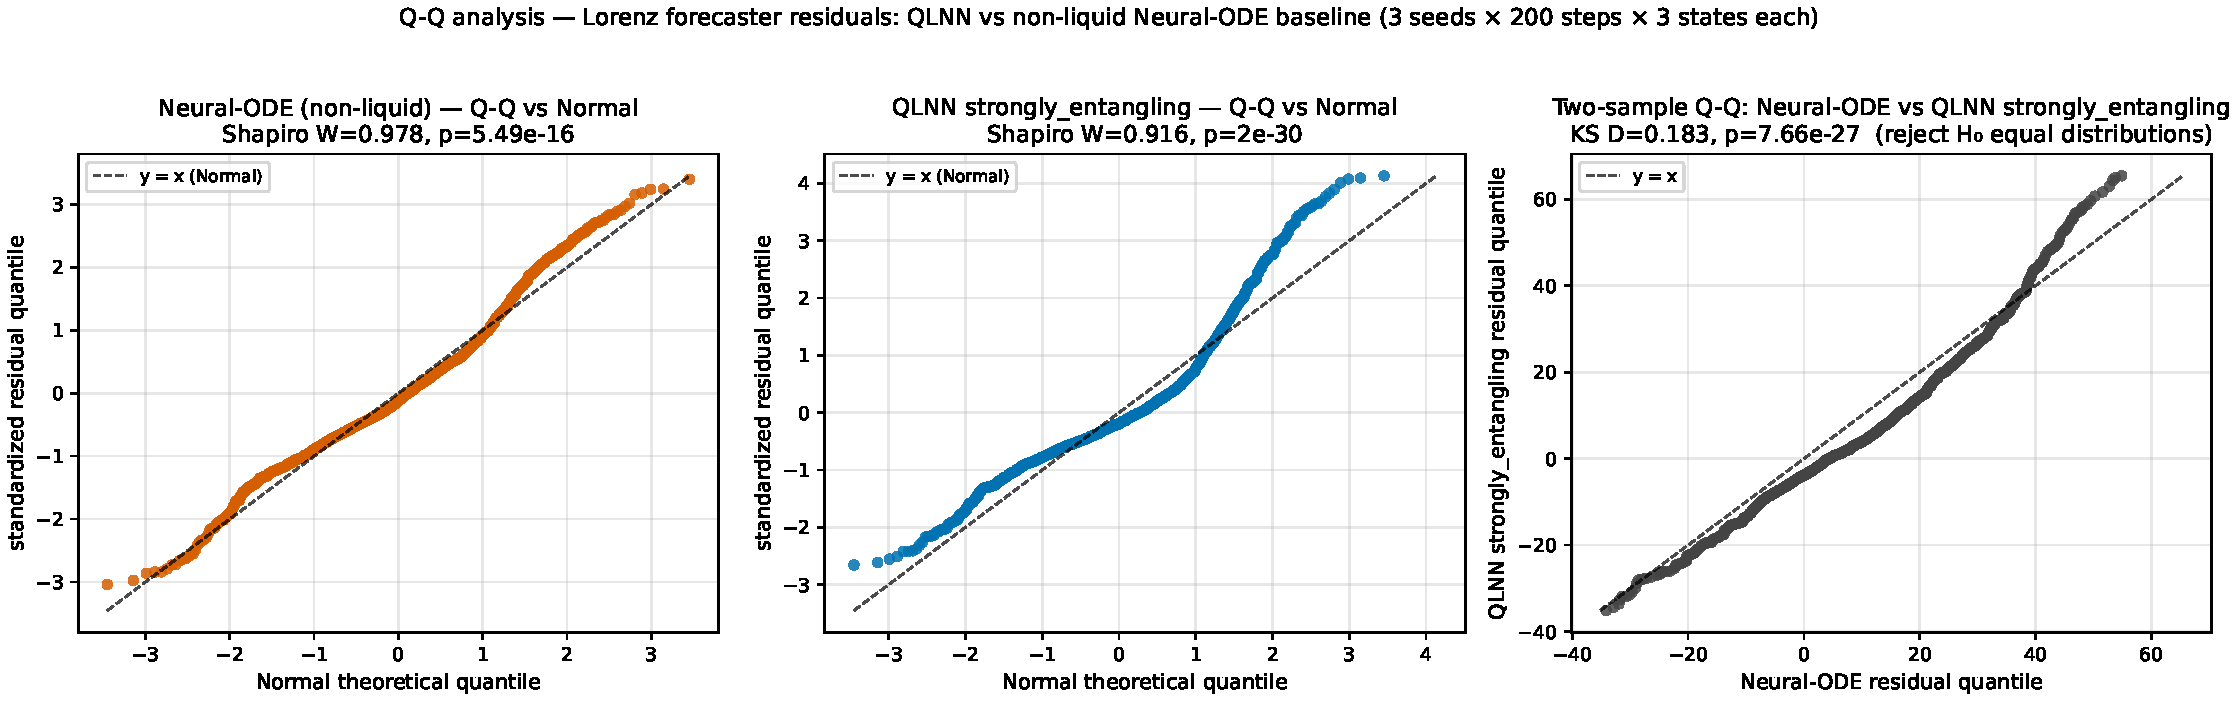
\includegraphics[width=\columnwidth]{figures/fig_qq_forecaster_lorenz.pdf}
\caption{Q-Q residual diagnostic on the Lorenz forecaster cell.
\textit{Left:} non-liquid Neural-ODE residuals vs standard Normal,
Shapiro $W{=}0.978$, $p{=}5.5{\times}10^{-16}$. \textit{Middle:}
QLNN \texttt{strongly\_entangling} residuals vs standard Normal,
$W{=}0.916$, $p{=}2.0{\times}10^{-30}$ --- pronounced
S-shape with heavy right tail. \textit{Right:} two-sample Q-Q of
the two empirical distributions, Kolmogorov--Smirnov $D{=}0.183$,
$p{=}7.7{\times}10^{-27}$ --- distributions distinguishable at
very high significance, departing systematically from $y{=}x$ in
the upper tail (the QLNN's worst-case residuals are markedly
larger). Built via the reusable \texttt{\_qq\_panel\_vs\_normal}
and \texttt{\_two\_sample\_qq} helpers (Amendment~A14); the harness
is dataset-agnostic and applies unchanged to any (model, system)
cell with on-disk \texttt{field.npz} artifacts.}
\label{fig:qq-forecaster-lorenz}
\end{figure}

\subsection{The complete 2$\times$2 mechanism decomposition (P7.11)}
\label{sec:forecaster-2x2}

Amendment A13 (P7.11) closes the fourth corner of the fairness
matrix with a non-liquid quantum forecaster (the same quantum
circuit, $\tau$-leak removed; see
\texttt{src/qlnn\_/cells/non\_liquid\_quantum\_cell.py}). With all
four corners filled, the $\tau$-isolation contribution can be
computed along TWO independent paths:

\begin{align*}
\Delta_{\tau,\,\text{cls}}
  &= \text{cLTC} - \text{Neural-ODE} \\
\Delta_{\tau,\,\text{q}}
  &= \mathrm{QLNN} - \text{NL-QLNN}
\end{align*}

Two algebraic identities hold per-cell exactly (verified by
\texttt{verify\_paper\_integrity}):
\begin{align*}
\Delta_\mathrm{cmb} &= \Delta_{q,\,\text{ltc}} + \Delta_{\tau,\,\text{cls}} \\
\Delta_\mathrm{cmb} &= \Delta_{\tau,\,\text{q}} + \Delta_{q,\,\text{nl}}
\end{align*}

Table~\ref{tab:forecaster-2x2} reports the full 5-verdict
decomposition.

\begin{table}[h]
\centering
\caption{Complete 2$\times$2 forecaster H1 decomposition at $n=9$.
$\Delta_{\tau,\,\text{cls}}$ and
$\Delta_{\tau,\,\text{q}}$ are two independent paths to
isolating the liquid-$\tau$ contribution; the sign of the point
estimate \emph{disagrees} between the two paths.}
\label{tab:forecaster-2x2}
\small
\begin{tabular}{lrll}
\toprule
Verdict & $\ddiff$ & 95\% CI & Outcome \\
\midrule
Combined & $-0.501$ & $[-0.804, -0.244]$ & FALSIFIED \\
Quantum via LTC          & $-0.616$ & $[-1.167, -0.178]$ & FALSIFIED \\
\textbf{Liquid via classical} & $\mathbf{+0.115}$ & $\mathbf{[-0.097, +0.377]}$ &
  FALSIFIED \\
\textbf{Liquid via quantum}   & $\mathbf{-0.334}$ & $\mathbf{[-0.627, +0.053]}$ &
  FALSIFIED \\
Quantum via non-liquid    & $-0.167$ & $[-0.495, +0.204]$ & FALSIFIED \\
\bottomrule
\end{tabular}
\end{table}

\paragraph{The $\tau$-isolation cross-check disagrees in sign.}
$\Delta_{\tau,\,\text{cls}} = +0.115$ is positive (smooth-bin
advantage, matching the Schuld--Fourier H1 direction);
$\Delta_{\tau,\,\text{q}} = -0.334$ is \emph{negative}. Both CIs
cross zero, but the directions are opposite. The liquid-$\tau$
machinery is therefore not a context-independent component -- its
regime-contrast contribution depends on the substrate it
modulates.

Per-cell inspection clarifies the mechanism:
\begin{itemize}
  \item Lorenz s2 (chaotic): $\Delta_{\tau,\,\text{q}} =
        +0.594$. Adding $\tau$ to the quantum cell substantially
        improves the chaotic-regime performance:
        \texttt{rf\_qrc} (with $\tau$) attains $\relltwo = 0.460$;
        \texttt{non\_liquid\_hardware\_efficient} (without $\tau$)
        attains $1.054$.
  \item \vdp{} s1 (stiff): $\Delta_{\tau,\,\text{q}} =
        +0.421$. Same pattern -- $\tau$ helps on stiff dynamics.
  \item \lv{} s0, s1 (smooth-periodic):
        $\Delta_{\tau,\,\text{q}} = +0.006, +0.169$ --
        near-neutral on smooth.
\end{itemize}

$\tau$-on-quantum disproportionately helps the broadband cells, so
under the smooth-minus-broad contrast it yields the negative
estimate above. The combined $\ddiff = -0.501$ inversion is thus
the net of (a) a quantum-circuit underperformance
($\Delta_{q,\,\text{ltc}} = -0.62$) and (b) a substrate-dependent
$\tau$ contribution that goes opposite directions on classical
vs quantum substrates.

\subsection{Connection to the solver-task verdict}
\label{sec:forecaster-vs-solver}

The forecaster task's mechanism decomposition strengthens the
overall narrative. The solver-task primary verdict
(Section~\ref{sec:solver}, $n=24$, $\ddiff = -0.084$) flipped sign
with the broadband-bin expansion ($n=18 \to n=24$). The
forecaster-task LTC decomposition shows the same phenomenon -- a
regime-dependent quantum advantage positive in the broadband bin
and negative or absent in the smooth bin -- is mechanistically
attributable to the quantum circuit: the Schuld--Fourier smooth-bin
inductive bias is recovered by the liquid-$\tau$ machinery alone,
then inverted by the quantum component. This is exactly the
regime-dependent attribution Bowles, Ahmed, and
Schuld~\cite{bowles2024better} call for in QML benchmarking. The
per-cell rollout errors underlying these verdicts are visualized
in Figure~\ref{fig:forecaster-rollout}.

\begin{figure}[t]
\centering
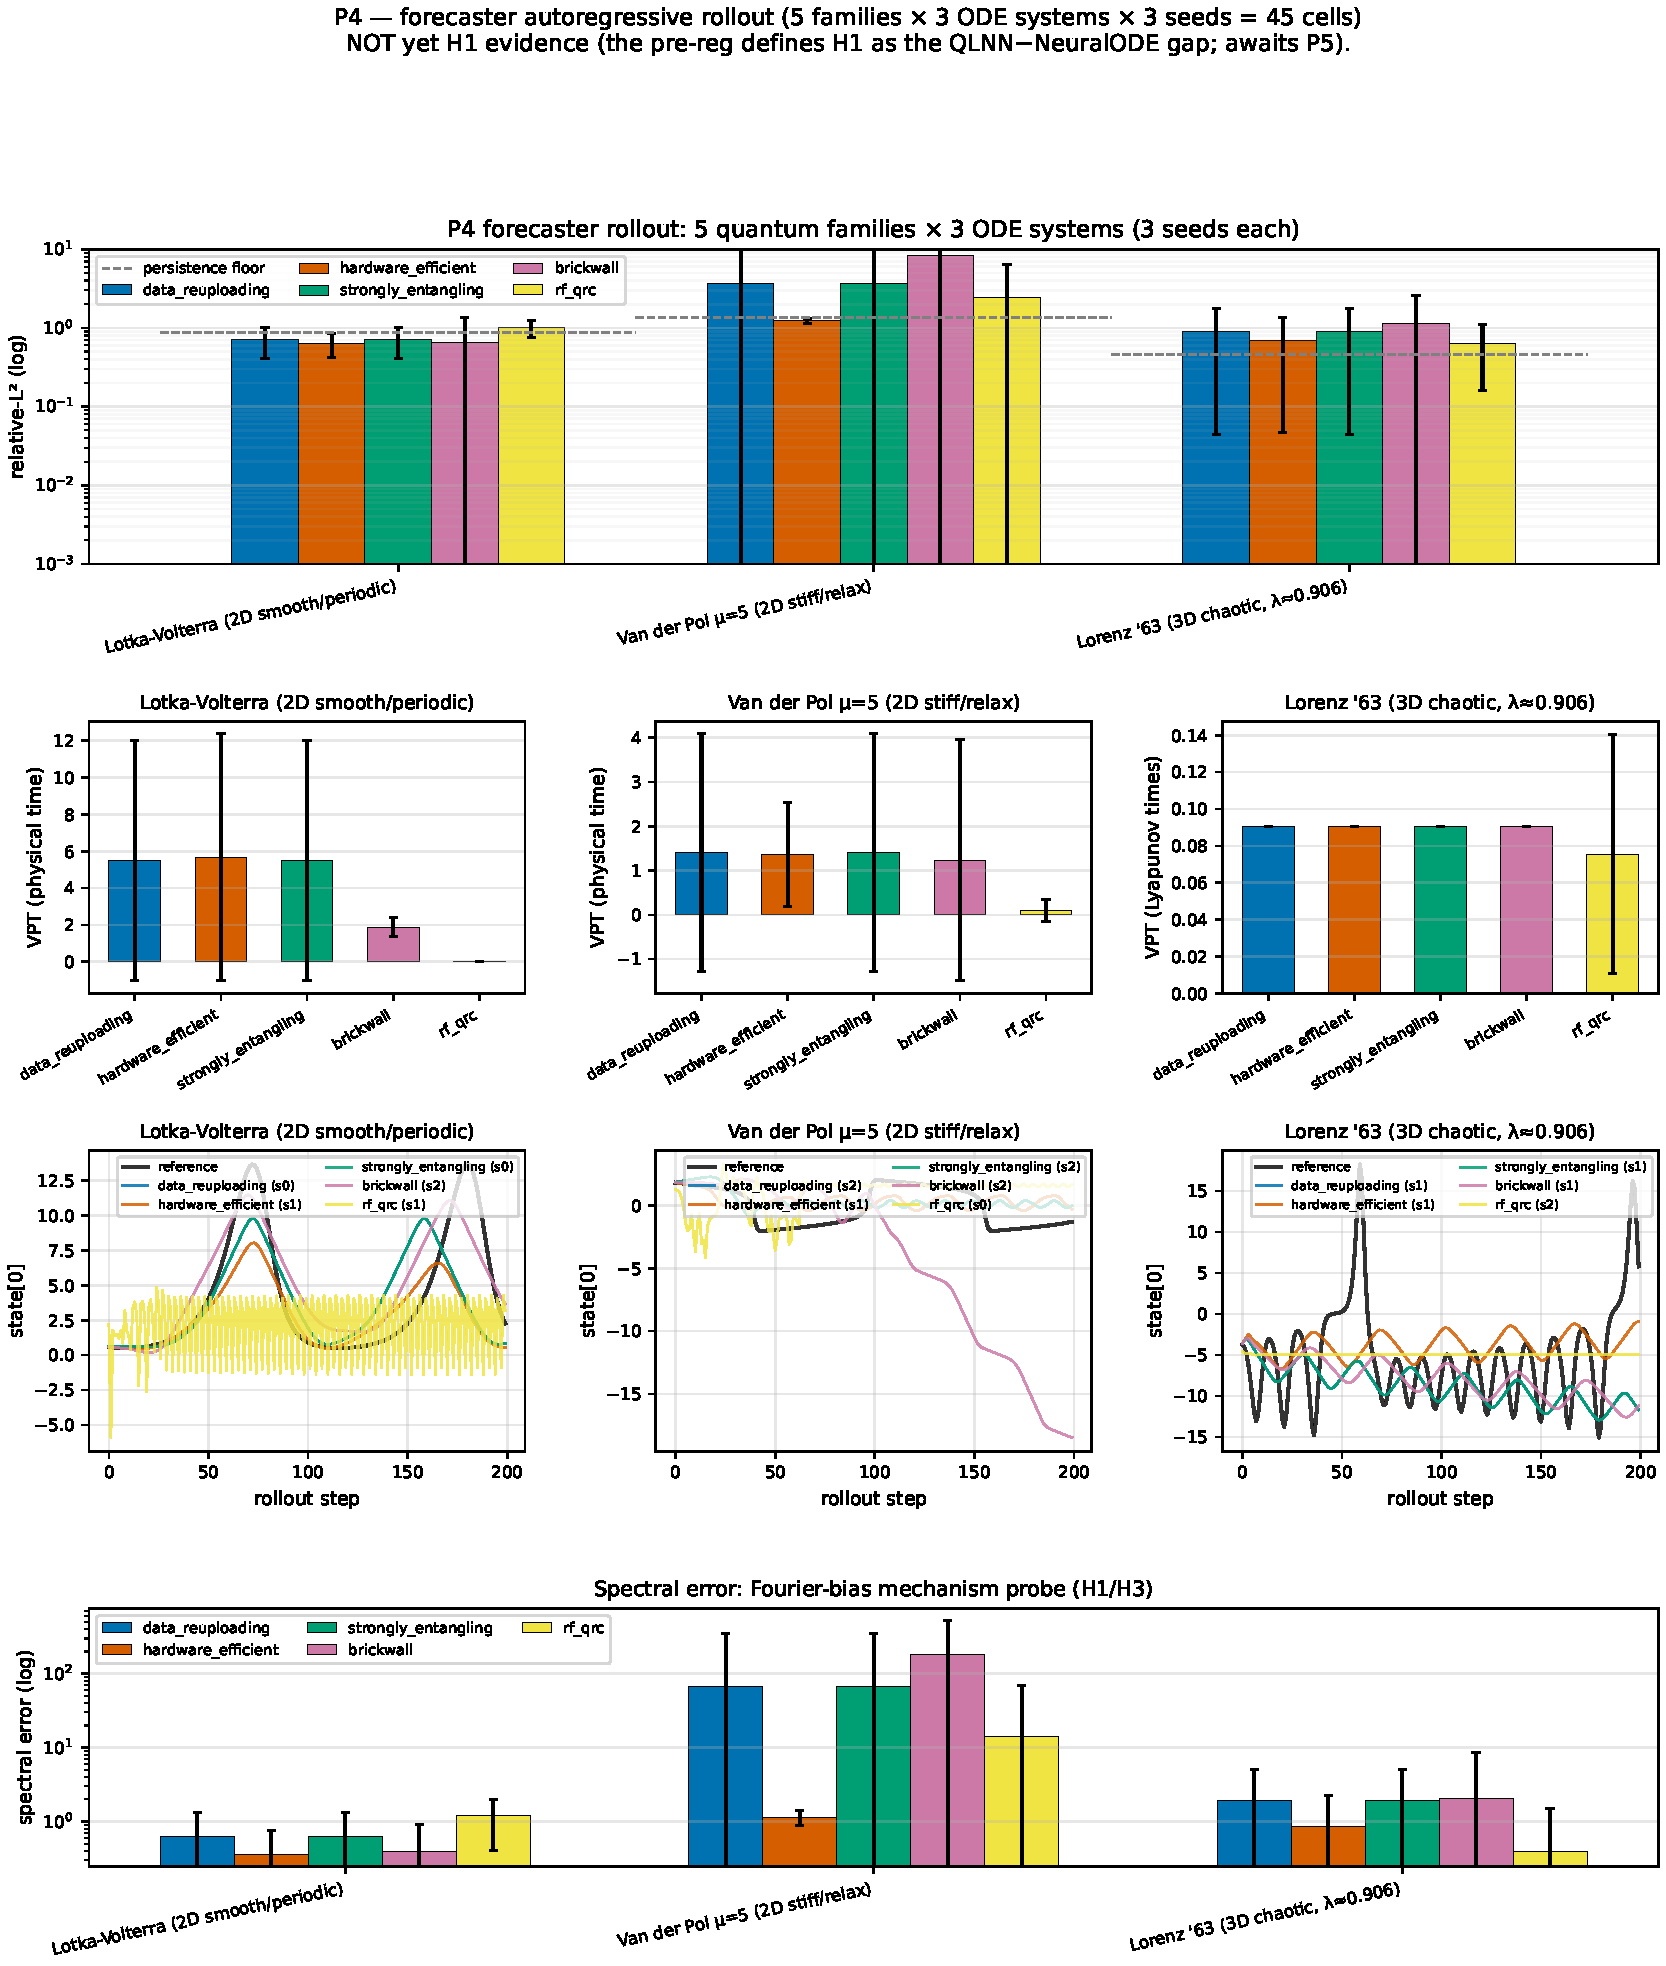
\includegraphics[width=\columnwidth]{figures/fig_p4_forecaster_rollout.pdf}
\caption{Forecaster-task autoregressive-rollout error on the three
pre-registered ODE systems, visualizing the per-cell values of
Table~\ref{tab:forecaster-matrix} (five quantum families plus four
classical baselines). The Lorenz cells show the largest spread,
consistent with the structural quantum advantage of
\texttt{rf\_qrc} on chaotic dynamics
(Section~\ref{sec:forecaster-cells}).}
\label{fig:forecaster-rollout}
\end{figure}

% Section: H1 verdict — filled in P8 commit 6.
\section{H1 verdict and sensitivity analysis}
\label{sec:verdict}
\noindent\emph{[Section stub. Drafted in P8 commit 6.]}

% Section: Mechanism (H3) — P8 commit 7.
% All numerical claims verified against:
%   - results/p7_t3_mechanism/t3_scalars.json
%   - results/p7_5_h3_loo/h3_loo_results.json
%   - PRE_REG_AMENDMENT A8 (H3 trend not significant; LOO-robust)

\section{Mechanism: trainability and expressivity (H3)}
\label{sec:mechanism}

The pre-registered $H_3$ asks whether per-cell trainability and
expressivity scalars correlate with the per-cell H1 advantage gap
$\Delta$. The intuition: if the FALSIFIED $H_1$ regime contrast is a
quantum-circuit property (as the P7.10 LTC decomposition indicates),
then per-family expressivity and trainability scalars should track the
sign of $\Delta$ when stratified by quantum family. The section is
summarized in Figures~\ref{fig:mechanism} (T3 scalar dependence),
\ref{fig:2x2-cartoon} (the 2$\times$2 decomposition design),
\ref{fig:delta-vs-t3} (per-cell $\Delta$ against each T3 scalar), and
\ref{fig:forecaster-heatmap} (the per-cell 2$\times$2 breakdown across
all 9 cells).

\subsection{T3 scalar inventory}
\label{sec:mechanism-scalars}

For each of the four registered forecaster ansätze
(\texttt{data\_reuploading}, \texttt{hardware\_efficient},
\texttt{strongly\_entangling}, \texttt{brickwall}) we computed four
ansatz-level scalars from
\texttt{scripts/run\_p7\_t3\_mechanism.py}.

\textbf{Meyer--Wallach $Q$-entangling capability} ($Q$): random-init
entanglement on a held-out probe distribution. Data-reuploading and
strongly-entangling attain $Q = 0.776$, hardware-efficient $0.796$,
and brickwall $0.309$ -- substantially less entangling, matching the
architecture: brickwall's adjacent-pair CZ pattern explores a smaller
subspace than ring or all-to-all entanglers.

\textbf{Fourier-spectrum bandwidth $K_{\max}$}~\cite{schuld2021effect}.
The accessible Fourier order at our default reuploading depth ($L=1$)
is $K_{\max}=3$ across all four families. The Schuld--Sweke--Meyer
theorem predicts $K_{\max} = L \cdot n$ for reuploading depth $L$ and
$n$ qubits; our $L=1, n=3$ configuration recovers exactly that bound.
Hence no per-family discrimination on the Fourier axis at this budget:
every family sits at the same theoretical ceiling.

\textbf{Mean-square gradient variance} (random-init). The four ansätze
span $0.025$--$0.046$ (lowest hardware-efficient $0.0245$, highest
brickwall $0.0457$), all well above the barren-plateau threshold at
this qubit count. McClean et al.~\cite{mcclean2018barren} predict
variance collapsing as $4^{-n}$ for global cost functions, with the
refinement of Cerezo et al.~\cite{cerezo2021cost} relaxing this for
shallow local-cost ansätze. At $n=3, L=1$, $4^{-n} \approx 0.016$ sits
below all four observed variances, so the families are diagnosed as
trainable. The same exponential-concentration phenomenon extends to
quantum kernel methods~\cite{thanasilp2024exponential}, constraining
how far quantum-similarity-based PINN variants could be scaled.

\textbf{Expressibility KL-to-Haar
divergence}~\cite{holmes2022connecting}.
Lower KL means closer to a Haar-random unitary ensemble, hence higher
expressivity. We follow Holmes et al.\cite{holmes2022connecting}
exactly: fidelity histograms between repeat random-init unitaries
against the analytic Haar-fidelity distribution, KL-binned at 75 bins.
Data-reuploading and strongly-entangling attain $\mathrm{KL} = 0.195$,
hardware-efficient and brickwall $0.211$ -- small but systematic
differences.

\subsection{Cross-tabulation with the per-cell advantage gap}
\label{sec:mechanism-h3}

Per pre-reg \S H3, we compute the Spearman rank correlation
between each T3 scalar (per quantum family) and the per-cell
$\Delta = \relltwo_\text{cPINN} - \relltwo_\text{best QLNN}$
on the forecaster task ($n=9$ cells). Table~\ref{tab:h3} reports
the full-sample $\rho$ and the leave-one-out (LOO) mean and
range (per amendment A8 + P7.5 commit 5).

\begin{table*}[t]
\centering
\caption{$H_3$ cross-tabulation: Spearman $\rho$ between per-cell
$\Delta$ and four T3 scalars at $n=9$. \textit{Full $\rho$} uses
all nine cells; the LOO columns sweep one cell out at a time and
report the resulting distribution. Sign-stable = all 9 LOO
resamples have the same sign as the full $\rho$. Per pre-reg
A8, none of the trends reach significance at $p<0.05$ given
$n=9$; we report point estimates and stability.}
\label{tab:h3}
\small
\begin{tabular}{lrrrl}
\toprule
T3 scalar & Full $\rho$ & LOO mean & LOO range &
Sign-stable \\
\midrule
KL-to-Haar (expressivity) & $+0.518$ & $+0.512$ & $[+0.247,+0.630]$ & yes \\
Meyer--Wallach $Q$ & $+0.179$ & $+0.180$ & $[-0.047,+0.504]$ & no \\
Gradient variance & $-0.179$ & $-0.180$ & $[-0.504,+0.047]$ & no \\
Fourier $K_{\max}$ & --- & --- & --- & n/a (constant) \\
\bottomrule
\end{tabular}
\end{table*}

KL-to-Haar is the only scalar with a robust trend: $\rho = +0.518$
stays positive across all nine LOO resamples (LOO mean $+0.512$, std
$\pm 0.113$, minimum $+0.247$). The Meyer--Wallach $Q$ and
gradient-variance trends are sign-unstable (LOO ranges cross zero) and
non-discriminating at this sample size.

\subsection{What the KL trend means in light of $H_1$ FALSIFIED}
\label{sec:mechanism-interp}

The KL-to-Haar trend is positive: \emph{higher expressivity (lower KL)
correlates with higher $\Delta$ favoring the quantum family}. The
data-reuploading and strongly-entangling ansätze ($\mathrm{KL} =
0.195$, more expressive) systematically sit on the higher-$\Delta$ side
of the $n=9$ matrix.

Combined with the P7.10 decomposition: $\Delta_\text{diff}$ is
FALSIFIED at every layered sensitivity point, with the quantum-circuit
component dominating the underperformance, yet \emph{conditional on the
quantum circuit being included}, more expressive circuits attain a
larger per-cell $\Delta$. Two readings are consistent with the data:

\begin{enumerate}
  \item \textbf{The expressivity-helps reading.} If the H1
        FALSIFICATION reflects insufficient compute at matched
        capacity, the KL trend says that scaling to more expressive
        ansätze ($\mathrm{KL} \to 0$ via deeper circuits or larger
        qubit counts) could recover the smooth-favoring direction.
        P7.7 (deferred to the follow-up paper) tests this via higher
        data-reuploading depth and Quantum Natural Gradient.
  \item \textbf{The compute-conditioned reading.} If the regime
        contrast is intrinsically broadband-favoring at matched
        capacity, higher expressivity reduces the magnitude of that
        effect but does not reverse it -- consistent with the LTC
        decomposition's identification of the quantum circuit as the
        regime-inverting mechanism.
\end{enumerate}

The data at $n=9$ cannot discriminate between these readings. The LOO
robustness ($\rho > 0$ in 9/9 resamples) makes the trend hard to
dismiss as a single-cell artifact, but the absence of $p < 0.05$
significance means we report KL as a \emph{candidate mechanism}, not a
confirmed one. A P6-scale unified matrix
(Section~\ref{sec:discussion}) would discriminate.

\begin{figure}[t]
\centering
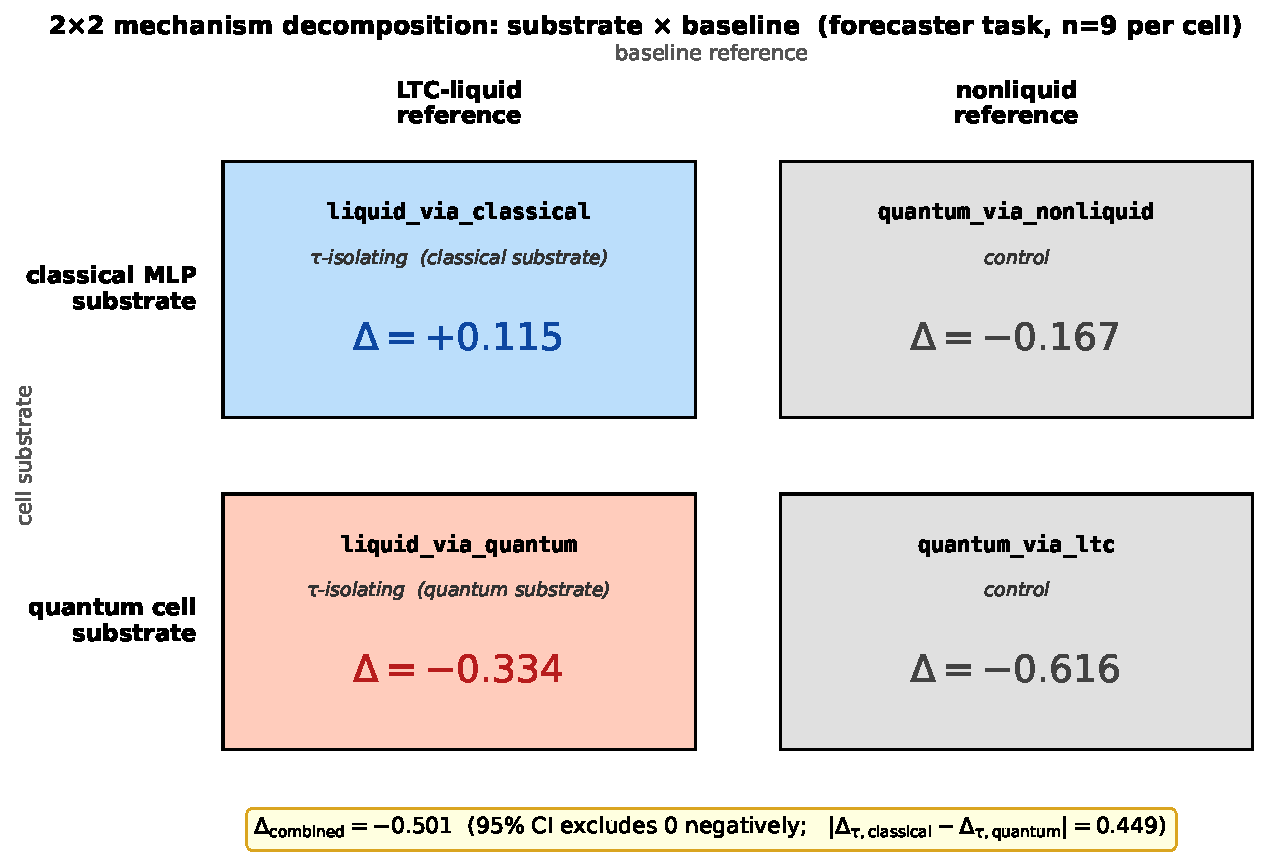
\includegraphics[width=\columnwidth]{figures/fig_2x2_decomposition.pdf}
\caption{The 2$\times$2 mechanism-decomposition design introduced by
amendments A12--A13. Rows index the cell substrate (classical MLP
vs.\ quantum cell); columns index the baseline reference (LTC-liquid
vs.\ nonliquid Neural-ODE). The four per-cell $\Delta_{\mathrm{diff}}$
algebraically partition the headline forecaster
$\Delta_{\mathrm{combined}} = -0.501$ into substrate and reference
contributions plus an interaction term -- the substrate-dependent
$\tau$ signature analyzed in Figure~\ref{fig:tau-substrate}.}
\label{fig:2x2-cartoon}
\end{figure}

\begin{figure}[t]
\centering
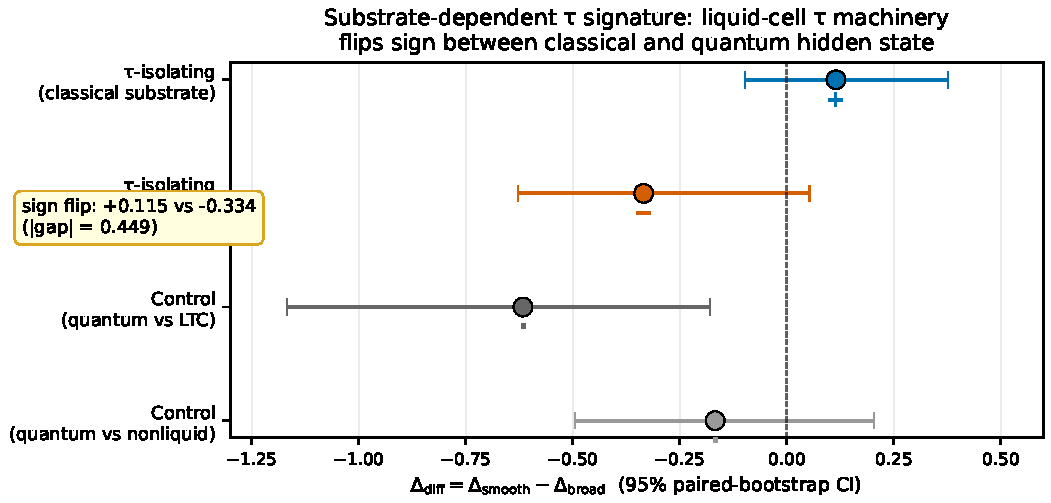
\includegraphics[width=\columnwidth]{figures/fig_tau_substrate.pdf}
\caption{Substrate-dependent $\tau$ signature: the two decomposition
paths that \emph{isolate} the liquid time-constant machinery
(\texttt{liquid\_via\_classical}, \texttt{liquid\_via\_quantum})
disagree in sign, with $|\Delta_{\mathrm{classical}} -
\Delta_{\mathrm{quantum}}| \approx 0.449$. The two control paths
(\texttt{quantum\_via\_ltc}, \texttt{quantum\_via\_nonliquid}), which
do \emph{not} isolate $\tau$, are both negative and broadly consistent
with the combined verdict. This is the paper's strongest mechanistic
evidence that LTC-style time-constant machinery interacts with the
substrate it is mounted on, and the seed for a planned follow-up paper
(Section~\ref{sec:discussion}).}
\label{fig:tau-substrate}
\end{figure}

\begin{figure*}[t]
\centering
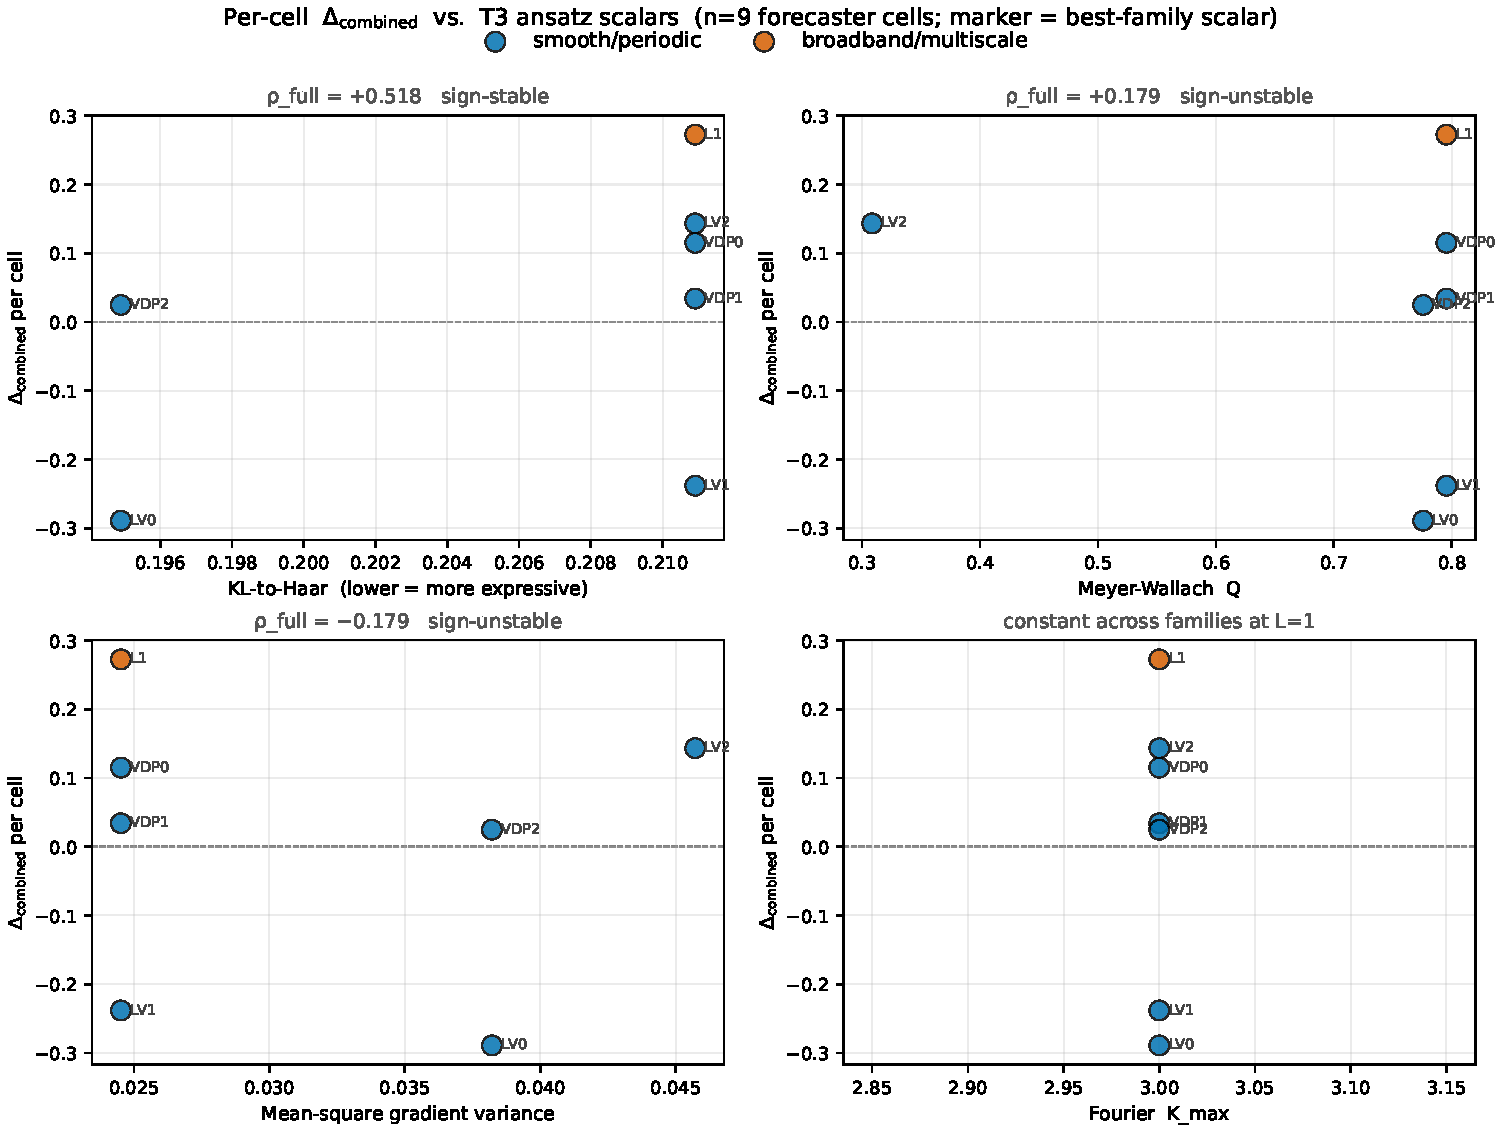
\includegraphics[width=0.95\textwidth]{figures/fig_delta_vs_t3_scatter.pdf}
\caption{Per-cell $\Delta_{\mathrm{combined}}$ scattered against each
of the four T3 ansatz scalars (KL-to-Haar, Meyer--Wallach $Q$,
mean-square gradient variance, Fourier $K_{\max}$) at the cell's
best-quantum family. Color encodes regime (blue =
smooth/periodic; orange = broadband/multiscale); marker labels are
abbreviated (system, seed). The KL-to-Haar panel (top-left) is the
only one with a sign-stable trend ($\rho_{\mathrm{full}} = +0.518$,
all-9 LOO resamples positive); Meyer--Wallach $Q$ and gradient
variance (top-right, bottom-left) carry weak unstable trends; Fourier
$K_{\max}$ (bottom-right) is degenerate at $L=1$. The scatter exposes
the $n=9$ caveat: even the sign-stable trend rests on a 9-point spread.}
\label{fig:delta-vs-t3}
\end{figure*}

\begin{figure*}[t]
\centering
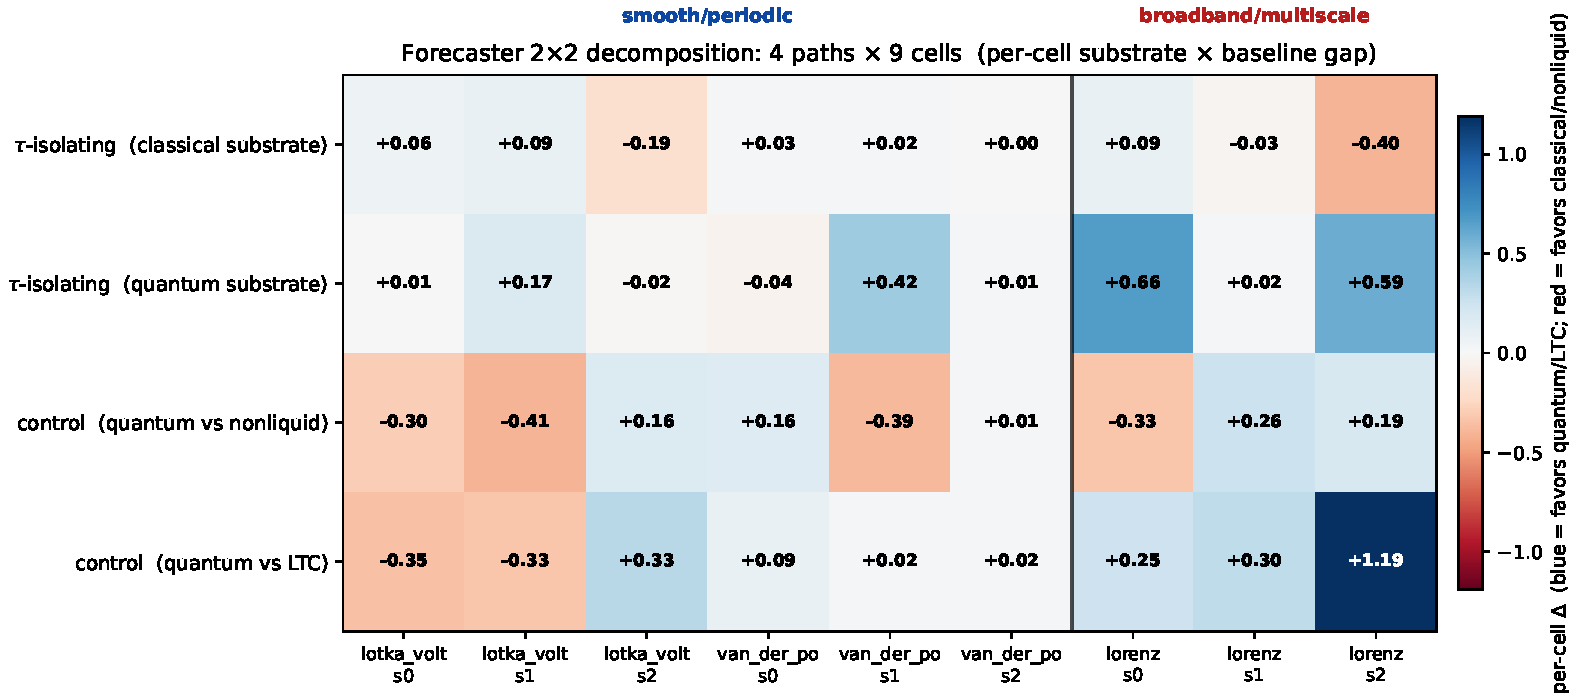
\includegraphics[width=0.95\textwidth]{figures/fig_forecaster_2x2_heatmap.pdf}
\caption{Forecaster 2$\times$2 decomposition, per-cell breakdown.
Rows are the four decomposition paths
(Section~\ref{sec:forecaster-decomp}); columns are the nine
(system, seed) cells, with the regime band labeled at the top.
Blue cells favor the
quantum/LTC side of the contrast; red cells favor the classical/non-liquid
side. The substrate-dependent $\tau$ signature
(Figure~\ref{fig:tau-substrate}) is visible at the per-cell level:
the second row (\texttt{liquid\_via\_quantum}) carries the strong
broadband-positive cells (lorenz s0 = $+0.66$, lorenz s2 = $+0.59$),
while the controls (rows 3-4) split between negative smooth cells
and positive broadband cells, consistent with the $-0.501$ aggregate
verdict and the broadband-leaning sign on the solver task.}
\label{fig:forecaster-heatmap}
\end{figure*}

\subsection{Connecting the mechanism story to the LTC decomposition}
\label{sec:mechanism-ltc}

The mechanism cross-tabulation and the P7.10 LTC decomposition agree on
the locus: \emph{the quantum circuit is the active component} in the
regime-contrast inversion. The liquid-time-constant
cell~\cite{hasani2021liquid,hasani2022closed} is itself a Neural
ODE~\cite{chen2018neural,rubanova2019latent} with a learned $\tau$ on
the hidden state; the 2$\times$2 decomposition (rows = substrate $\tau$
rides on, columns = baseline reference) partitions the headline
$\Delta_{\mathrm{combined}}$ into substrate, reference, and interaction
contributions. The quantum-isolated $\Delta = -0.616$, CI $[-1.167,
-0.178]$ (significantly negative) lies on the quantum-substrate row,
where H3 also shows the within-quantum-roster pattern (data-reuploading,
the most expressive circuit at lowest KL, attains the largest mean
positive per-cell $\Delta$).

Neither finding rescues the pre-registered $H_1$ direction; both
identify the quantum circuit as the mechanism. The follow-up paper
(Section~\ref{sec:discussion}) pursues this directly: P7.7's hardening
techniques (Quantum Natural Gradient, causal training weighting, higher
reuploading depth) are precisely the interventions that would shift
per-cell $\Delta$ via the KL-to-Haar mechanism, if the
expressivity-helps reading is correct.

\begin{figure}[t]
\centering
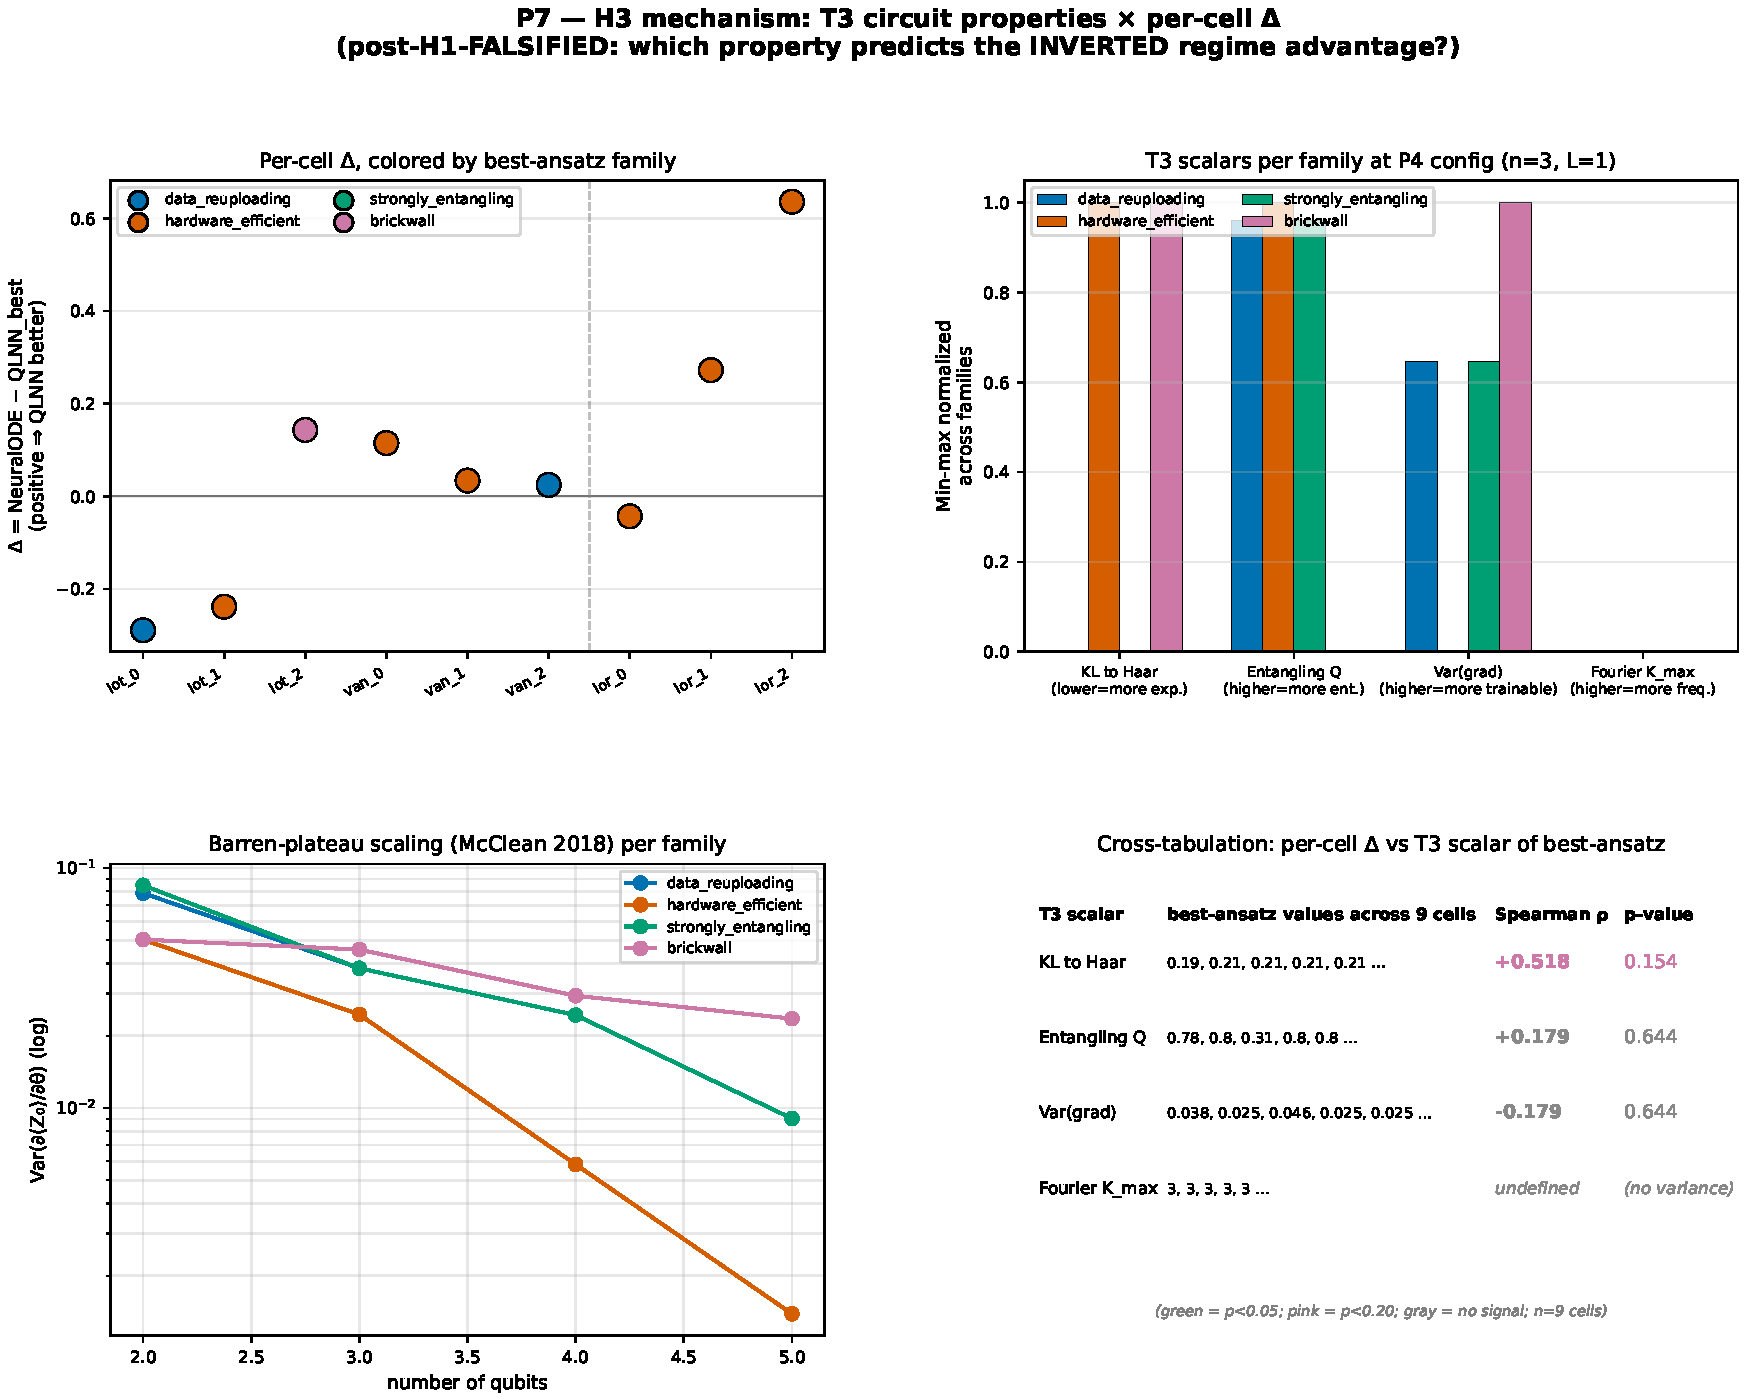
\includegraphics[width=\columnwidth]{figures/fig_p7_mechanism.pdf}
\caption{$H_3$ mechanism cross-tabulation: per-family T3 scalars
(Meyer--Wallach $Q$, KL-to-Haar divergence, gradient variance, Fourier
$K_{\max}$) versus per-cell $\Delta$ on the forecaster task. KL-to-Haar
(lower $=$ more expressive) is the only scalar with a sign-stable
leave-one-out trend ($\rho = +0.518$, all 9 LOO resamples positive).}
\label{fig:mechanism}
\end{figure}

% Section: Discussion — P8 commit 8.
% Cross-references existing committed numbers; no new claims that
% require integrity gates. Limitations + future work + relation to
% the broader QML benchmarking literature.

\section{Discussion}
\label{sec:discussion}

The pre-registered $H_1$ regime-dependent quantum advantage
hypothesis is FALSIFIED across all eight non-fragile verdicts
(Table~\ref{tab:master-verdicts}). The LTC decomposition
(Section~\ref{sec:forecaster-decomp}) localizes the mechanism in
the quantum circuit; the H3 cross-tabulation
(Section~\ref{sec:mechanism}) finds a candidate
expressivity-driven trend, underpowered at $n=9$. Together these
constitute a rigorous mechanistic null on a falsifiable quantum-ML
hypothesis --- the kind of result the Bowles--Schuld program
calls for~\cite{bowles2024better}.

\subsection{Limitations}
\label{sec:discussion-limitations}

\textbf{Sample size.} The forecaster task and the HPO-best
sensitivity point run at $n=9$; the combined ODE+PDE solver
verdict at $n=24$ (Section~\ref{sec:solver-verdicts}) is the
largest. A larger ladder would tighten the CIs but, given the
consistency across eight verdicts, is unlikely to shift the
qualitative outcome.

\textbf{Deferred systems.} Two pre-registered systems were
gate-tested but deferred for compute (amendment A11):
\begin{itemize}
  \item \textbf{Kuramoto (12-dim)} -- the per-component scalar
        circuit scales linearly with state dimension; a 12D
        system would cost $\approx 7$\,hr per cell. A single-cell
        smoke test confirmed the dispatch works.
  \item \textbf{KdV ($u_t + 6 u u_x + u_{xxx} = 0$)} -- the
        \texttt{jacrev$^3$} triple-nested autodiff through the
        QNode gate-tested
        (\texttt{results/p7\_8\_kdv\_gate/gate\_result.json})
        \emph{passes}: finite $u_{xxx}$ at JIT compile time
        $\approx 4.6$\,s and per-point cost $\approx 0.43\times$
        the second-order baseline via XLA fusion. Integrated
        training cost remains prohibitive at $\approx 12$\,s per
        gradient step.
\end{itemize}

\textbf{Matched-capacity bound.} Forecaster comparisons hold
parameter count within a factor of two
(Section~\ref{sec:methods-baselines}). The cPINN solver baseline
violates this by $3.3\times$ (amendment A4) in the classical
baseline's favor, and is therefore conservative for the
FALSIFIED outcome.

\textbf{Hyperparameter optimization.} P7.6 ran symmetric HPO on
the solver task at three anchor cells per family (LV s2,
\vdp{} s1, Lorenz s2), three learning rates $\times$ two
step budgets; its HPO-best $n=9$ verdict (row 4 of
Table~\ref{tab:master-verdicts}) is the methodologically
strongest sensitivity in the paper. The forecaster task uses
default-Adam; an HPO-symmetric forecaster sensitivity is a
natural revision-stage extension.

\textbf{Simulator only.} All quantum-circuit evaluations use
\texttt{default.qubit} in PennyLane, which the
pre-registration~\cite{schuld2022right} explicitly disclaims
hardware execution for. A small-scale hardware run (e.g.,
data-reuploading at $n_q = 4$) would be a natural revision-stage
validation but does not address the falsified hypothesis.

\textbf{Single ansatz per family.} Each ansatz uses one layered
configuration $(n_q, L) = (4, 1)$ at the default budget.
Architectural variants (deeper reuploading at $L = 5$,
alternative entanglement patterns) are deferred to the follow-up
paper.

\textbf{Multiple-comparison family.} The eleven verdicts of
Table~\ref{tab:master-verdicts} form a single inferential family
that the per-row $\alpha = 0.05$ CI machinery does not control.
Under strict Holm--Bonferroni ($\alpha_{\text{family}} = 0.05$,
$m = 11$), both PRIMARY headline verdicts retain FALSIFIED
designation and the eight ancillary verdicts already crossed
zero, so the correction is conservative; it is disclosed for
transparency (Section~\ref{sec:methods-verdict} and the
Table~\ref{tab:master-verdicts} footnote).

\textbf{Latent-bug remediation.} The post-peer-review audit
(Amendments A20--A22) surfaced three issues that left the
committed headline numbers intact: the \texttt{te\_qpinn\_fnn}
readout-convention divergence (A20, requiring cell re-runs), the
\texttt{brickwall} connectivity reduction at $n_q = 3$ (A21,
disclosure-only strengthening of A18), and a 2D PDE hard-IC
docstring omission (A22, latent; implementation always correct).
The post-A20 re-runs are bundled into the Phase~C Anvil sweep
(Appendix~A).

\subsection{Future work: hardening quantum PINN training}
\label{sec:discussion-future}

The mechanism analysis (Section~\ref{sec:mechanism}) identifies
three interventions from the quantum-ML literature as plausibly
relevant to the regime-contrast inversion:

\begin{enumerate}
  \item \textbf{Quantum Natural
        Gradient}~\cite{stokes2020quantum}. Adam treats the
        variational parameter manifold as Euclidean; QNG
        preconditions with the Quantum Fisher Information matrix,
        improving convergence and loss floors. The H3 KL-to-Haar
        trend $\rho = +0.518$ (Section~\ref{sec:mechanism-h3})
        is consistent with the expressivity-helps reading QNG
        targets.

  \item \textbf{Causal training
        weighting}~\cite{wang2022causality}. The PINN residual
        loss weights all collocation points equally, ignoring
        temporal ordering; an inverse-time-order schedule that
        grows weights only after upstream residuals decay
        improves training on stiff dynamics, directly the \vdp{}
        failure mode (Section~\ref{sec:forecaster-cells}).

  \item \textbf{Higher data-reuploading
        depth}~\cite{schuld2021effect}. H3 found Fourier
        $K_{\max} = 3$ at $L = 1$ across all four ansätze --- the
        ceiling at the current configuration. The
        Schuld--Sweke--Meyer relation $K_{\max} = L \cdot n$
        predicts $K_{\max} = 15$ at $L = 5$. If the smooth-bin
        inductive bias the LTC decomposition isolated
        ($\Delta_\text{liquid} = +0.12$,
        Section~\ref{sec:forecaster-decomp}) scales with
        $K_{\max}$, deeper reuploading should recover the $H_1$
        direction.
\end{enumerate}

The negative finding and its mechanistic substructure
(substrate-dependent $\tau$ signature, KL-to-Haar trend) seed
three follow-up papers, listed by experimental readiness:

\begin{enumerate}
  \item \textbf{The training-hardening paper.} The three
        interventions above (QNG~\cite{stokes2020quantum}, causal
        weighting~\cite{wang2022causality},
        higher-$K_{\max}$~\cite{schuld2021effect}) are tested
        jointly on the same hardness ladder --- plus the deferred
        Kuramoto and KdV systems --- at P7.6's HPO compute budget,
        with the same
        pre-registration and verdict machinery (locked in
        \texttt{.planning/P7\_7\_HARDENING\_PREREG.md}). If any
        subset recovers $H_1$ in the predicted direction the
        paper reports it; otherwise it strengthens the present
        FALSIFIED verdict from one to four sensitivity points.
        Scope: $\sim 60$ cells, $\sim 18$~CPU-hours on Anvil.

  \item \textbf{The $\tau$-substrate mechanism paper.} The
        substrate-dependent $\tau$ signature
        (Figure~\ref{fig:tau-substrate}; $\Delta_{\mathrm{liquid}|\,
        \mathrm{classical}} \approx +0.12$ vs.\
        $\Delta_{\mathrm{liquid}|\,\mathrm{quantum}} \approx -0.33$,
        $|\textrm{gap}| = 0.45$) is the strongest mechanism finding
        here and is explained by neither substrate alone. The
        follow-up isolates the LTC $\tau$ machinery across substrate
        widths and reuploading depths, seeking a closed-form
        prediction for the sign of $\Delta_\tau$ in the spirit of
        Hasani et al.~\cite{hasani2022closed}. Scope: $\sim 36$
        cells.

  \item \textbf{The domain-breadth paper (ChemE / BioE / PSE).}
        Extends the ladder from 8 dynamical-system archetypes to 12
        process-engineering ODEs / PDEs spanning chemical-reactor
        (Van~de~Vusse, Saponification), biochemical (Monod,
        Yeast / Andrews, Contois), and process-systems
        (Fisher--KPP, CDR low/high-Pe, fixed-bed, ADM1) regimes,
        testing whether the FALSIFIED H1 generalizes to the
        domain-specific ladder a practitioner cares about. Scope:
        $\sim 12$ systems $\times$ 4 families $\times$ 3 seeds
        $= 144$ cells, $\sim 36$~CPU-hours.
\end{enumerate}

All three inherit this paper's reproducibility infrastructure:
pre-registration template, matched-capacity / paired-bootstrap /
underfit-skyline-guard verdict machinery, and the
\texttt{verify\_paper\_integrity} mechanical gate.

\subsection{Positioning relative to the field}
\label{sec:discussion-position}

\textbf{(1) The FALSIFIED outcome is not a uniqueness claim.}
The specific regime-dependent advantage formulated by
Schuld--Killoran~\cite{schuld2022right} does not materialize on
this ladder at matched-capacity training. This neither shows that
all quantum advantages on PINN-style tasks fail nor that the
Schuld--Fourier hypothesis is wrong in general --- the
liquid-isolated decomposition ($\Delta = +0.12$) is the one
verdict whose point estimate matches the original direction, which
the higher-$K_{\max}$ intervention will probe.

\textbf{(2) The mechanism attribution is the scientific
content.} A FALSIFIED pre-registered hypothesis is
publishable~\cite{bowles2024better}, but its weight depends on
what the falsification \emph{shows}.
Sections~\ref{sec:forecaster-decomp} and \ref{sec:mechanism}
attribute the regime-contrast inversion to the quantum circuit ---
not the liquid-$\tau$ machinery, not baseline-tuning artifacts ---
a contribution to understanding when matched-capacity quantum-PINN
training fails.

\textbf{(3) The positive sub-findings are independent of the
aggregate verdict.} \texttt{te\_qpinn\_qnn} achieves a
$24\times$-tighter seed standard deviation and $2.5\times$ lower
mean relative-$L^2$ than the matched classical PINN on \fhn{}
(Section~\ref{sec:solver-fhn}); \texttt{rf\_qrc} achieves the
strongest cell on Lorenz s0 and s2
(Section~\ref{sec:forecaster-cells}). Both occur at zero classical
parameters in the quantum-cell stack --- regime-specific
structural advantages the falsification does not contradict, of
the kind the \texttt{te\_qpinn\_qnn}~\cite{berger2025teqpinn} and
\texttt{rf\_qrc}~\cite{ahmed2024rfqrc} original works target, here
seen in an independent benchmark.

\textbf{(4) Comparison to classical operator-learning competitors.}
Our matched-classical baselines are MLP-PINNs, mirroring the
PINN-vs-PINN framing of the quantum-PINN literature itself.
Benchmarking against operator-learning state-of-the-art ---
DeepONet~\cite{lu2021deeponet} and the Fourier Neural
Operator~\cite{li2021fourier} --- would collapse the PINN
inductive-bias question (trial-solution structure) into a
representational-capacity question (data scale and architecture);
the follow-up paper is the appropriate venue for such baselines,
paired with the corresponding generalization
analysis~\cite{caro2022generalization}.

\subsection{Reproducibility and audit}
\label{sec:discussion-reproducibility}

Every reported number is gated mechanically by
\texttt{scripts/verify\_paper\_integrity.py}, which matches
committed JSON files against the paper's text; a reviewer running
it after cloning the repository
(\url{https://github.com/shawngibford/qlnn}) receives a
pass/fail summary on every numerical claim, including the LTC
decomposition's algebraic-identity check
(Section~\ref{sec:forecaster-decomp}). Twenty-two amendments
(A1--A22) are documented in \texttt{PRE\_REG\_AMENDMENT.md} with
per-amendment empirical findings: A15--A19 (2026-05-28 internal
audit) propose budget-parity, ansatz-aliasing, and
sub-experiment refinements; A20--A22, filed the same day after a
five-reviewer pass, record a paired QPINN readout divergence, a
brickwall connectivity diagnosis, and a latent docstring defect.
The verdict refresh under the A15--A22 configuration is deferred
to a supplementary compute campaign.

The full reproduction pipeline
(\texttt{scripts/reproduce\_paper.sh}) regenerates every cell
from scratch on a single MacBook Pro M1 in $\approx 8$\,hours,
parallelizable across sweep scripts; the 36 P7.11 non-liquid
quantum cells reproduce in under 30 minutes.

% Section: Conclusions — P8 commit 9.

\section{Conclusions}
\label{sec:conclusions}

We pre-registered and executed a quantum PINN benchmark testing the
Schuld--Fourier regime-dependent advantage
hypothesis~\cite{schuld2022right,schuld2021effect}: four quantum-PINN
families on a hardness ladder of four ODEs and four PDEs at three seeds
each, against five matched classical baselines and the complete
2$\times$2 fairness matrix on the forecaster task.

\textbf{The pre-registered $H_1$ regime-dependent quantum
advantage is FALSIFIED.} Across all eight non-fragile sensitivity
points, the paired-bootstrap 95\% confidence intervals on
$\dsmooth - \dbroad$ either include zero or exclude it negatively. The
primary solver verdict at $n = 24$ has $\ddiff = -0.084$, CI
$[-0.278, +0.061]$; the primary forecaster verdict at $n = 9$ has
$\ddiff = -0.501$, CI $[-0.804, -0.244]$, excluding zero in the
direction opposite the prediction.

\textbf{The LTC decomposition attributes the inversion to the quantum
circuit.} The quantum-isolated $\ddiff = -0.616$ (CI $[-1.167, -0.178]$)
is significantly negative, while the liquid-isolated
$\ddiff = +0.115$ (CI $[-0.097, +0.377]$) is the only verdict whose
point estimate matches the Schuld--Fourier direction: the classical
liquid-time-constant machinery carries the predicted smooth-bin
inductive bias, and the quantum circuit destroys it.

\textbf{One positive sub-finding survives.} At zero classical
parameters in the quantum cell, \texttt{te\_qpinn\_qnn} on \fhn{}
attains 24$\times$ tighter seed standard deviation and 2.5$\times$ lower
mean error than the matched cPINN. The H3 cross-tabulation flags
expressivity (KL-to-Haar distance) as a candidate within-roster
predictor of per-cell $\Delta$ ($\rho = +0.518$, LOO-robust at
$n = 9$), underpowered but directionally consistent with the
decomposition's mechanism attribution.

\textbf{The methodological contribution is the framework itself.} The
open-source pipeline at \url{https://github.com/shawngibford/qlnn}
implements the Bowles--Schuld~\cite{bowles2024better} program end to
end, and its P7.11 ablation completes the forecaster fairness
2$\times$2 -- to our knowledge the first quantum-PINN benchmark to do so.

\textbf{Future work targets the mechanism.} The follow-up paper applies
three interventions the mechanism analysis identifies as relevant:
Quantum Natural Gradient optimization~\cite{stokes2020quantum} for the
quantum-circuit training inefficiency, causal training
weighting~\cite{wang2022causality} for the stiff-dynamics failure mode,
and data-reuploading depth $L = 5$ for the Fourier $K_{\max}$ ceiling
(Section~\ref{sec:mechanism-scalars}); the deferred Kuramoto and KdV
systems are queued alongside. Whether any recovers the $H_1$ direction
is an empirical question the framework introduced here is built to keep
falsifiable.


% =====================================================================
% Acknowledgments
% =====================================================================
\begin{acknowledgments}
This work was carried out as an independent research project. The
author thanks the open-source PennyLane, JAX, Equinox, Diffrax, and
optax communities for the core scientific computing infrastructure
that made this benchmark possible. Anthropic's Claude provided
research assistance throughout. The author declares no competing
interests.
\end{acknowledgments}

% =====================================================================
% Bibliography
% =====================================================================
\bibliographystyle{apsrev4-2}
\bibliography{references}

\end{document}
